\documentclass[%
%%% PARA ESCOLHER O ESTILO TIRE O SIMBOLO %(COMENTÁRIO)
%SemVinculoColorido,
%SemFormatacaoCapitulo,
%SemFolhaAprovacao,
%SemImagens,
%CitacaoNumerica, %% o padrão é citação tipo autor-data
%PublicacaoDissOuTese, %% (é também o "default") com ficha catal. e folha de aprovação em branco. Caso tenha lista de símbolos e lista de siglas e abreviaturas retirar os comentários dos arquivos siglas.tex e abreviaturasesiglas.tex. Retirar também os comentários indicados nesse arquivo, nos includes
%PublicacaoArtigoOuRelatorio, %% texto sequencial, sem quebra de páginas nem folhas em branco
PublicacaoProposta, %% igual tese/dissertação, mas sem ficha catal. e fol. de aprov.
%PublicacaoLivro, %% com capítulos
%PublicacaoLivro,SemFormatacaoCapitulo, %% sem capítulos
%english,portuguese %% para os documentos em Português com abstract.tex em Inglês
portuguese,english %% para os documentos em Inglês com abstract.tex em Português
,LogoINPE% comentar essa linha para fazer aparecer o logo do Governo (Ex.: LogoINPE usado em ano eleitoral). Caso deseje alterar o logo governo verificar a pasta .template/logo/logoverno.png
,CCBYNC	% as opções de licença são: CCBY, CCBYSA, CCBYND, CCBYNC, CCBYNCSA, CCBYNCND, GPLv3 e INPECopyright
]{./template/tdiinpe}
%\documentclass[english,portuguese,LogoINPE,CCBYNC]{http://urlib.net/iconet.com.br/banon/2008/03.25.01.19/tdiinpe}

% PARA EXIBIR EM ARIAL TIRAR O COMENTÁRIO DAS DUAS LINHAS SEGUINTES
%\renewcommand{\rmdefault}{phv} % Arial
%\renewcommand{\sfdefault}{phv} % Arial

%%%%%%%%%%%%%%%%%%%%%%%%%%%%%%%%%%%%%%%%%%%%%
%%% Pacotes já previamente carregados:      %
%%%%%%%%%%%%%%%%%%%%%%%%%%%%%%%%%%%%%%%%%%%%%%%%%%%%%%%%%%%%%%%%%%%%%%%%
%%% ifthen,calc,graphicx,color,inputenc,babel,hyphenat,array,setspace, %
%%% bigdelim,multirow,supertabular,tabularx,longtable,lastpage,lscape, %
%%% rotate,caption2,amsmath,amssymb,amsthm,subfigure,tocloft,makeidx,  %
%%% eso-pic,calligra,hyperref,ae,fontenc                               %
%%%%%%%%%%%%%%%%%%%%%%%%%%%%%%%%%%%%%%%%%%%%%%%%%%%%%%%%%%%%%%%%%%%%%%%%
%%% insira neste campo, comandos de LaTeX %%%
%%% \usepackage{_exemplo_}
% etc.
%%%%%%%%%%%%%%%%%%%%%%%%%%%%%%%%%%%%%%%%%%%%%

%\watermark{Revisão No. ##} %% use o comando \watermark para identificar a versão de seu documento
%% comente este comando quando for gerar a versão final
\usepackage{rotating}
\usepackage{dsfont}
\usepackage{comment}
%%%%%%%%%%%%%%%%%%%CAPA%%%%%%%%%%%%%%%%%%%%%%%%%%%%%%%%
%\serieinpe{INPE-NNNNN-TDI/NNNN} %% não mais usado

%\titulo{Data-driven Parameter Discovery of One-dimensional Burgers' Equation Using Physics-Informed Neural Network}
\titulo{Implementation of the ecRad Radiation Module Using Physics Informed Machine Learning}
%\title{Descoberta de parâmetros baseada em dados da equação de Burguers unidimensional usando rede neural informada pela física} %% 
\title{Implementação do Módulo de Radiação ecRad Usando Aprendizado de Máquina Informado pela Física} %% 
\author{Eduardo F. Miranda}
\descriccao{Exame de Proposta de Doutorado do Curso de Pós-Graduação em Computação Aplicada, orientada pelos Dr. Stephan Stephany e Dr. Roberto Pinto Souto aprovada em 27 de agosto de 2024.}
\repositorio{aa/bb/cc/dd} %% repositório onde está depositado este documento - na omissão, será preenchido pelo SID
\tipoDaPublicacao{TDI}	%% tipo da publicação (NTC, RPQ, PRP, MAN, PUD, TDI, TAE e PRE) na ausência do número de série INPE, caso contrário deixar vazio
\IBI{xx/yy} %% IBI (exemplo: J8LNKAN8PW/36CT2G2) quando existir, caso contrário o nome do repositório onde está depositado o documento

\date{2024}%ano da publicação

%%%%%%%%%%%%%%%%%%%%%%%%%%VERSO DA CAPA%%%%%%%%%%%%%%%%%%%%%%%%%%%%%%%%%%%%%%%%%%%%%%%
\tituloverso{\vspace{-0.9cm}\textbf{\PublicadoPor:}}
\descriccaoverso{Instituto Nacional de Pesquisas Espaciais - INPE\\
Coordenação de Ensino, Pesquisa e Extensão (COEPE)\\
Divisão de Biblioteca (DIBIB)\\
CEP 12.227-010\\
São José dos Campos - SP - Brasil\\
Tel.:(012) 3208-6923/7348\\
%Fax: (012) 3208-6919\\
E-mail: {pubtc@inpe.br}
}
\descriccaoversoA{\textbf{\ConselhoDeEditoracao:}\\
\textbf{\Presidente:}\\
Dra. Marley Cavalcante de Lima Moscati -  Coordenação-Geral de Ciências da Terra (CGCT)\\
\textbf{\Membros:}\\
Dra. Ieda Del Arco Sanches - Conselho de Pós-Graduação (CPG)\\
Dr. Evandro Marconi Rocco - Coordenação-Geral de Engenharia, Tecnologia e Ciência Espaciais  (CGCE)\\
Dr. Rafael Duarte Coelho dos Santos - Coordenação-Geral de Infraestrutura e Pesquisas Aplicadas (CGIP)\\
Simone Angélica Del Ducca Barbedo - Divisão de Biblioteca (DIBIB)\\
\textbf{\BibliotecaDigital:}\\
Dr. Gerald Jean Francis Banon \\
Clayton Martins Pereira - Divisão de Biblioteca (DIBIB)\\
%Jefferson Andrade Ancelmo - Divisão de Biblioteca (DIBIB)\\
%Simone A. Del-Ducca Barbedo - Divisão de Biblioteca (DIBIB)\\
%Deicy Farabello - Centro de Previsão de Tempo  e Estudos Climáticos (CGCPT)\\
\textbf{\RevisaoNormalizacaoDocumentaria:}\\
Simone Angélica Del Ducca Barbedo - Divisão de Biblioteca (DIBIB) \\
%Marilúcia Santos Melo Cid - Divisão de Biblioteca (SID)\\
%Yolanda Ribeiro da Silva Souza - Divisão de Biblioteca (DIBIB)\\
André Luis Dias Fernandes - Divisão de Biblioteca (DIBIB)\\
\textbf{\EditoracaoEletronica:}\\
Ivone Martins - Divisão de Biblioteca (DIBIB)\\
André Luis Dias Fernandes - Divisão de Biblioteca (DIBIB)\\
}

%%%%%%%%%%%%%%%%%%%FOLHA DE ROSTO

%%%%%%%%%%%%%%%FICHA CATALOGRÁFICA
%% NÃO PREENCHER - SERÁ PREENCHIDO PELO SID

\cutterFICHAC{Cutter}
\autorUltimoNomeFICHAC{Sobrenome, Nomes} %% exemplo: Fuckner, Marcus André
\autorFICHAC {Nome Completo do Autor1; Nome Completo do Autor2} %% Campo opcional (se não usado prevalece \author)
\tituloFICHAC{Titulo da publicação}
\instituicaosigla{INPE}
\instituicaocidade{São José dos Campos}
\paginasFICHAC{\pageref{numeroDePáginasDoPretexto} + \pageref{LastPage}} %% número total de páginas
%\serieinpe{INPE-00000-TDI/0000} %% não mais usado
\palavraschaveFICHAC{1.~Palavra chave. 2.~Palavra chave 3.~Palavra chave. 4.~Palavra chave. 5.~Palavra chave  I.~\mbox{Título}.} %% recomenda-se pelo menos 5 palavras-chaves - \mbox{} é para evitar hifenização 
\numeroCDUFICHAC{000.000} %% número do CDU 

% Nota da ficha (para TD)
\tipoTD{Dissertação ou Tese} % Dissertação ou Tese
\cursoFA{Mestrado ou Doutorado em Nome do Curso}
\instituicaoDefesa{Instituto Nacional de Pesquisas Espaciais}
\anoDefesa{AAAA} % ano de defesa 
\nomeAtributoOrientadorFICHAC{Orientador}	% pode ser: Orientador, Orientadora ou Orientadores
\valorAtributoOrientadorFICHAC{José da Silva} % nome(s) completo(s)

%%%%%%%%%%%%%%%FOLHA DE APROVAÇAO PELA BANCA EXAMINADORA
\tituloFA{\textbf{ATENÇÃO! A FOLHA DE APROVAÇÃO SERÁ INCLUIDA POSTERIORMENTE.}}
%\cursoFA{\textbf{}}
\candidatoOUcandidataFA{}
\dataAprovacaoFA{}
\membroA{}{}{}
\membroB{}{}{}
\membroC{}{}{}
\membroD{}{}{}
\membroE{}{}{}
\membroF{}{}{}
\membroG{}{}{}
\ifpdf

%%%%%%%%%%%%%%NÍVEL DE COMPRESSÃO {0 -- 9}
\pdfcompresslevel 9
\fi
%%% define em 80% a largura das figuras %%%
\newlength{\mylenfig} 
\setlength{\mylenfig}{0.8\textwidth}
%%%%%%%%%%%%%%%%%%%%%%%%%%%%%%%%%%%%%%%%%%%

%%%%%%%%%%%%%%COMANDOS PESSOAIS
%\newcommand{\vetor}[1]{\mathit{\mathbf{#1}}}



\graphicspath{{docs/img/}}  %#ef

\hbadness=10000
\vbadness=10000


\usepackage{microtype}  %#ef

\usepackage{lipsum}  %#ef

\usepackage{listings}  %#ef
% \makeatletter
% \let\@ORGmakecaption\@makecaption
% \long\def\@makecaption#1#2{\@ORGmakecaption{#1}{#2}\vskip\belowcaptionskip\relax}
% \makeatother
\lstdefinestyle{mystyle}{
frame               = single,
rulecolor           = \color{gray},
basicstyle          = \ttfamily\small,
belowcaptionskip    = 8pt,
aboveskip           = 8pt,
belowskip           = 8pt,
columns             = fullflexible,
breakatwhitespace   = false,
breaklines          = true,
keepspaces          = true,
showspaces          = false,
showstringspaces    = false,
inputencoding       = utf8,
extendedchars       = true,
literate            =
{á}{{\'a}}1 {é}{{\'e}}1 {í}{{\'i}}1 {ó}{{\'o}}1 {ú}{{\'u}}1
{Á}{{\'A}}1 {É}{{\'E}}1 {Í}{{\'I}}1 {Ó}{{\'O}}1 {Ú}{{\'U}}1
{à}{{\`a}}1 {è}{{\`e}}1 {ì}{{\`i}}1 {ò}{{\`o}}1 {ù}{{\`u}}1
{À}{{\`A}}1 {È}{{\'E}}1 {Ì}{{\`I}}1 {Ò}{{\`O}}1 {Ù}{{\`U}}1
{ä}{{\"a}}1 {ë}{{\"e}}1 {ï}{{\"i}}1 {ö}{{\"o}}1 {ü}{{\"u}}1
{Ä}{{\"A}}1 {Ë}{{\"E}}1 {Ï}{{\"I}}1 {Ö}{{\"O}}1 {Ü}{{\"U}}1
{â}{{\^a}}1 {ê}{{\^e}}1 {î}{{\^i}}1 {ô}{{\^o}}1 {û}{{\^u}}1
{Â}{{\^A}}1 {Ê}{{\^E}}1 {Î}{{\^I}}1 {Ô}{{\^O}}1 {Û}{{\^U}}1
{œ}{{\oe}}1 {Œ}{{\OE}}1 {æ}{{\ae}}1 {Æ}{{\AE}}1 {ß}{{\ss}}1
{ç}{{\c c}}1 {Ç}{{\c C}}1 {ø}{{\o}}1 {å}{{\r a}}1 {Å}{{\r A}}1
{€}{{\EUR}}1 {£}{{\pounds}}1 {ã}{{\~a}}1 {Ã}{{\~A}}1,
showtabs=false,
tabsize=2,
}
\lstset{}  %#ef
\lstset{style=mystyle}  %#ef

\usepackage{xurl}  %#ef

\usepackage{enumitem} %#ef  % http://ctan.org/pkg/enumitem

\usepackage{placeins}  %#ef  % floatbarrier




% PARA PUBLICAÇÕES EM INGLÊS:
%% Descomentar essa linha para publicações em inglês
\bibliographystyle{./template/abnt-alfenglish}

% PARA PUBLICAÇÕES EM PORTUGUÊS:
%% comentar essa linha para publicações em inglês
%\bibliographystyle{./template/abnt-alfportuguese}

 %% faça as modificações pertinentes no arquivo configuracao.tex

\makeindex  %% não alterar, gera INDEX, caso haja algum termo indexado no texto

\begin{document} %% início do documento %% não mexer

%\marcaRegistrada{}	% comando opcional usado para informar abaixo da ficha catalográfica sobre marca registrada
\marcaRegistrada{Informar aqui sobre marca registrada (a modificação desta linha deve ser feita no arquivo publicacao.tex).}
%\financiamento{}	% comando opcional usado para informar abaixo da ficha catalográfica sobre fontes financiadoras
\financiamento{Informar aqui sobre fontes financiadoras (a modificação desta linha deve ser feita no arquivo publicacao.tex).}
%\financiamento{O presente trabalho foi realizado com apoio da Coordenação de Aperfeiçoamento de Pessoal de Nível Superior - Brasil (CAPES) - Código de Financiamento 001.}
%\financiamento{This study was financed in part by the Coordenação de Aperfeiçoamento de Pessoal de Nível Superior - Brasil (CAPES) - Finance Code 001.}

\maketitle  %% não alterar, gera páginas obrigatórias (folha de rosto, ficha catalográfica e folha de aprovação), automaticamente

%%% Comente as linhas opcionais abaixo caso não as deseje
%\include{./docs/01_epigrafe} %% Opcional
% \include{./docs/02_dedicatoria} %% Opcional
% \include{./docs/03_agradecimentos} %% Opcional
%%%%%%%%%%%%%%%%%%%%%%%%%%%%%%%%%%%%%%%%%%%%%%%%%%%%%%%%%%%%%%%%%%%%%%%%%%%%%%%%
% RESUMO %% obrigatório
\begin{resumo}
%% neste arquivo resumo.tex
%% o texto do resumo e as palavras-chave têm que ser em Português para os documentos escritos em Português
%% o texto do resumo e as palavras-chave têm que ser em Inglês para os documentos escritos em Inglês
%% os nomes dos comandos \begin{resumo}, \end{resumo}, \palavraschave e \palavrachave não devem ser alterados
%\hypertarget{estilo:resumo}{} %% uso para este Guia


% -------------------------------------- OLD 2024-08-01
% This thesis aims to exploit a physics-informed machine learning implementation of the ecRad radiation module used in a numerical model of the European Centre for Medium-Range Weather Forecasts (ECMWF). Such implementation may use a physics-based neural network, an approach already exploited for a simpler problem, the solving of the 1D Burger's equation. In this thesis proposal, a Deep Neural Network (DNN) was implemented, but it is not physics-informed. 

% Former work about the 1D Burger's equation presented the use of a data-driven parameter discovery for a Partial Differential Equation (PDE) using a Physics-Informed Neural Network (PINN). This approach is then compared to some standard numerical models for parameter discovery. The 1D Burgers' equation is a PDE with spatial and temporal derivatives, which is generally solved by a numerical model. Recent studies proposed the use of a Deep Neural Network (DNN) for solving a PDE or for data-driven parameter discovery of the PDE. In any case, the training phase of DNN requires a high number of sample points in order to obtain accurate solutions. In this way, PINNs, which are DNN embedding underlying physical equations as prior knowledge, were proposed in order to make feasible the use of a lower number of sample points in the training phase. Usually, the physical equations are used in the PINN loss function. Similarly to any DNN, PINNs can also be considered universal function approximators. The accuracy and computation times related to the estimation of the 1D Burgers' equation were discussed.


% -------------------------------------- OLD 2024-08-22
%This thesis aims to explore Physics-Informed Machine Learning (PIML) alternatives for the ecRad radiation module used at the European Centre for Medium-Range Weather Forecasts (ECMWF). Such an implementation could employ a Physics-Informed Neural Network (PINN), an approach already used for a simpler problem, solving the one-dimensional (1D) Burgers' Equation. In this thesis proposal, a Deep Neural Network (DNN) was implemented, but not physics-informed.

%Preliminary work addressed data-driven parameter discovery for a Partial Differential Equation (PDE) using a PINN. This approach was then compared with some standard numerical models for parameter discovery. The chosen test problem was the one-dimensional (1D) Burgers' Equation, a PDE with spatial and temporal derivatives, usually solved by a numerical model. Recent studies have proposed the use of some DNN to solve a PDE or for data-driven discovery of PDE parameters. In any case, the training phase of the DNN requires a large number of sample points to obtain accurate solutions. Consequently, PINNs, which are DNNs that incorporate underlying physical equations as prior knowledge, were proposed in order to enable the use of a smaller number of sample points in the training phase. Usually, physical equations are used in the PINN loss function. For the Burgers Equation, the accuracy and processing time to estimate the equation parameters are discussed. For the radiation module, the root mean square error (RMSE) of the heating rate and the processing time of ecRad are discussed.


This thesis demonstrates the use of a Machine Learning (ML) approach to optimize part of the ecRad radiation module employed in numerical weather and climate models, which is implemented using a numerical algorithm and is very computationally demanding. The ecRad radiation module is employed in an operational model of the European Centre for Medium-Range Weather Forecasts (ECMWF), but in this work, it will be developed and tested as a stand-alone implementation. The gas-optical scheme of the radiation module would be replaced by a ML-based implementation, following the current trend applied to model standard microphysics modules. In particular, it is intended to explore Physics-Informed Machine Learning (PIML) alternatives for the gas-optical scheme, starting with a former class of PIML methods, the Physics-Informed Neural Networks (PINNs). However, preliminary work has already been carried out for the gas-optical scheme using a ML approach implemented by a Deep Neural Network (DNN), reproducing the work of some authors. An incremental approach is then proposed for the thesis, starting with a non-PIML DNN, followed by a PINN implementation, and then exploring other PIML implementations. A previous of this thesis work applied a PINN approach to a simpler problem related to the one-dimensional Burgers' Equation, modeled by a partial differential equation. Test results and analyses are presented here for both previous works. An additional point is how to integrate the ML code, implemented in the Python environment and its associated libraries, with the ecRad radiation module written in Fortran 90.




\palavraschave{%
	\palavrachave{Physics-informed Machine Learning}%
    \palavrachave{Radiation Module}%
	\palavrachave{Deep Neural Network}%
	\palavrachave{Physics-informed Neural Network}%
	\palavrachave{High Performance Computing}%
}
 
\end{resumo} %% obrigatório
%%%%%%%%%%%%%%%%%%%%%%%%%%%%%%%%%%%%%%%%%%%%%%%%%%%%%%%%%%%%%%%%%%%%%%%%%%%%%%%%
% ABSTRACT
\begin{abstract}
%% neste arquivo abstract.tex
%% o texto do resumo e as palavras-chave têm que ser em Inglês para os documentos escritos em Português
%% o texto do resumo e as palavras-chave têm que ser em Português para os documentos escritos em Inglês
%% os nomes dos comandos \begin{abstract}, \end{abstract}, \keywords e \palavrachave não devem ser alterados
%\selectlanguage{english}	%% para os documentos escritos em Português
\selectlanguage{portuguese}	%% para os documentos escritos em Inglês
%\hypertarget{estilo:abstract}{} %% uso para este Guia

%Esta tese objetiva explorar alternativas de Aprendizado de Máquina Informado pela Física (\textit{Physics-Informed Machine Learning}, PIML) para o módulo de radiação ecRad usado no European Centre for Medium-Range Weather Forecasts (ECMWF). Tal implementação pode empregar uma Rede Neural Informada pela Física (\textit{Physics-Informed Neural Network}, PINN), uma abordagem já utilizada para um problema mais simples, a resolução da Equação de Burgers unidimensional (1D). Nesta proposta de tese, uma Rede Neural Profunda (\textit{Deep Neural Network}, DNN) foi implementada, mas não informada pela física.

%Trabalhos preliminares abordaram descoberta de parâmetros baseada em dados para uma Equação Diferencial Parcial (EDP) usando uma PINN. Esta abordagem foi então comparada com alguns modelos numéricos padrão para descoberta de parâmetros. O problema-teste escolhido foi a Equação de Burgers unidimensional (1D), uma EDP com derivadas espaciais e temporais, geralmente resolvida por modelo numérico. Estudos recentes propuseram o uso de alguma DNN para resolver uma EDP ou para descoberta de parâmetros da EDP baseada em dados. De qualquer forma, a fase de treinamento da DNN requer um elevado número de pontos amostrais para obter soluções precisas. Consequentemente, PINNs, que são DNNs que incorporam equações físicas subjacentes como conhecimento prévio, foram propostos a fim de viabilizar a utilização de uma quantidade menor de pontos amostrais na fase de treinamento. Geralmente as equações físicas são usadas na função de perda da PINN. Para a Equação de Burgers, a precisão e o tempo de processamento para estimar os parâmetros da equação são discutidos. O erro quadrático médio (\textit{Root Mean Square Error}, RMSE) da taxa de aquecimento e o tempo de processamento do ecRad são discutidos.


Esta tese demonstra o uso de uma abordagem de aprendizado de máquina para otimizar parte do módulo de radiação ecRad empregado em modelos numéricos de previsão de tempo de clima, o qual emprega um algoritmo numérico que requer muito processamento. O módulo de radiação ecRad é usado num modelo operacional do European Centre for Medium-Range Weather Forecasts (ECMWF), mas neste trabalho será desenvolvido e testado como uma implementação independente. O esquema gás-ótico do módulo de radiação será substituído por uma implementação baseada em aprendizado de máquina, seguindo a tendência atual aplicada a módulos padrão da microfísica de modelos. Em particular, pretende-se explorar alternativas de Physics-Informed Machine Learning (PIML) para o esquema gás-ótico, começando com uma classe inicialmente proposta de métodos PIML, as Physics-Informed Neural Networks (PINNs). Entretanto, um estudo preliminar já foi desenvolvido para o esquema gás-ótico usando uma abordagem de aprendizado de máquina implementado por uma rede neural profunda (Deep Neural Network - DNN), reproduzindo o trabalho de alguns autores. Uma abordagem incremental é então proposta para a tese, começando com a DNN, fora do escopo de PIML, seguida de uma abordagem PINN e depois explorando outras classes de métodos PIML. Outro trabalho preliminar da tese aplicou uma abordagem PINN para um problema mais simples relacionado à equação unidimensional de Burgers, que é modelada por uma equação diferencial parcial. Resultados de testes e análises são apresentados aqui para ambos esses trabalhos preliminares. Um ponto adicional é como integrar o código de aprendizado de máquina, implementado no ambiente Python e suas bibliotecas associadas, com o módulo de radiação ecRad escrito em Fortran 90.


\palavraschave{%
	\palavrachave{Aprendizado de Máquina Informado pela Física}%
	\palavrachave{Módulo de Radiação}%
    \palavrachave{Rede Neural Profunda}%
	\palavrachave{Rede Neural Informada pela Física}%
	\palavrachave{Processamento de Alto Desempenho}%
}

%\selectlanguage{portuguese}	%% para os documentos escritos em Português
\selectlanguage{english}	%% para os documentos escritos em Inglês
\end{abstract} %% obrigatório

\includeListaFiguras %% obrigatório caso haja mais de 3 figuras, gerado automaticamente
\includeListaTabelas %% obrigatório caso haja mais de 3 tabelas, gerado automaticamente

% \include{./docs/06_abreviaturasesiglas} %% opcional %% altere o arquivo siglaseabreviaturas.tex
% \include{./docs/07_simbolos} %% opcional %% altere o arquivo simbolos.tex

\includeSumario  %% obrigatório, gerado automaticamente

\inicioIntroducao %% não altere este comando

%========================================
\chapter{INTRODUCTION}
\label{ch:intr}
%========================================

This thesis aims to explore Physics-Informed Machine Learning (PIML) alternatives to replace part of the ecRad radiation numerical module, which is used by the global weather and climate model Integrated Forecasting System (IFS) of the European Centre for Medium-Range Weather Forecasts (ECMWF). The IFS model was developed and maintained jointly by the ECMWF, based in Reading, England, and Météo-France, based in Toulouse, France. PIML is described in \autoref{sec:piml}, while the initial class of Physics-Informed Neural Networks (PINN) methods is described in \autoref{sec:pinn}. The ecRad radiation module appears in \autoref{sec:ers}. Former work in this thesis research included a PINN implementation for a test case, shown in this document. The objectives of this thesis are then shown in \autoref{sec:otr}.

%========================================
\section{Physics-Informed Machine Learning (PIML) }
\label{sec:piml}
%========================================

PIML is a set of methods and tools that systematically integrate Machine Learning (ML) algorithms with physical constraints and mathematical models developed in scientific and engineering domains. As opposed to purely data-driven methods, PIML models can be trained from additional information obtained by enforcing physical laws such as energy and mass conservation. More broadly, PIML models can include abstract properties and conditions such as stability, convexity, or invariance. The basic premise of PIML is that the integration of ML and physics can yield more effective, physically consistent, and data-efficient models. Recent advances in PIML for dynamical system modeling and control includes: (i) physics-informed learning for system identification; (ii) physics-informed learning for control; (iii) analysis and verification of PIML models; and (iv) physics-based digital twin, which consists of parameterized components whose physical properties can be altered to provide data from source systems that are identical to the target system
\cite{Nghiem2023}.

According to \citeonline{Karniadakis2021}, despite great progress in simulating multiphysics problems using the numerical discretization of partial differential equations (PDEs), one still cannot seamlessly incorporate noisy data into existing algorithms, mesh generation remains complex, and high-dimensional problems governed by parameterized PDEs cannot be tackled. Moreover, solving inverse problems with hidden physics is often prohibitively expensive and requires different formulations and elaborate computer codes. In this context, ML emerges as a promising alternative, being a current research thread. However, training deep neural networks may require big data, which is not always available for scientific problems. Instead, such networks can be trained from additional information obtained by enforcing the physical laws, for example, at random points in the continuous space-time domain. Such physics-informed learning integrates noiseless or noisy data and mathematical models implemented by neural networks or other ML methods. Moreover, it may be possible to design specialized network architectures that automatically satisfy some of the physical invariants for better accuracy, faster training and improved generalization. Considering PIML approaches, some of the prevailing trends, capabilities and limitations in embedding physics into ML are discussed. Some PIML applications both for forward and inverse problems are presented, including discovering hidden physics and tackling high-dimensional problems.

PIML is a methodology that improves model accuracy and interpretability by combining physics concepts and ML techniques, enables more robust predictions while reducing the need for large amounts of training data, and has numerous potential applications in science and engineering, such as modeling physical systems, solving partial differential equations, and performing inverse analysis and optimization. Some approaches used in PIML can be classified as: physics-constrained ML, physics-guided ML, physics-encoded ML, data augmentation through physics principles, transfer learning from physics-based synthetic data to experimental data, and delta-learning physics correction to improve physics generalization and delta-learning unknown physics to represent unmodeled physical phenomena \cite{Tronci2024}. In addition, there is also a need for new PIML standardized frameworks and patterns, as well as new PIML approaches, to enable scalable and robust implementations. 

A first PIML approach was given by the Physics-Informed Neural Networks (PINN), which employ DNN for problems related to the solving of Partial Differential Equation (PDE), as described below.


%========================================
\section{Physics-Informed Neural Networks}
\label{sec:pinn}
%========================================

Previous work related of this thesis research evaluated the parameter discovery of the data-driven one-dimensional Burgers' Equation (1D Burgers) using a PINN implementation. 

Concerning PINNs, many simulations are mathematically modeled by PDEs, which have derivatives in space and time. Typically, the coefficients of these derivatives are unknowns that express physical properties of the problem being modeled by the PDE, which is usually solved by standard Numerical Models (NM) like the finite difference method. Recent work has proposed to solve a PDE, or discover the parameters of the PDE based on data, using Deep Neural Network (DNN). The universal approximation theorem states that a DNN can approximate any continuous function, as long as the network has a sufficient number of hidden layers and employs nonlinear activation functions \cite{Hornik1989}. In any case, for parameter resolution or discovery, depending on the architecture employed, the DNN training input is provided by sample points, which compose a subset of the full set of known points of the function in the space and time domain. These sample points can be conveniently selected in order to increase its number of data related to initial (IC) and boundary conditions (BC). These sample points are then called Collocation Points (CP) \cite{Basdevant1986}, a name that came from standard NMs. 

However, either for solving a PDE or for  parameter discovery of the PDE, the training phase of DNN requires a high number of sample points in order to obtain accurate solutions. Sample points can be obtained either by observation or using synthetic data from a known model. PINNs, which are DNN embedding underlying physical equations as prior knowledge, were proposed in order to make feasible the use of a lower number of sample points in the training phase \cite{Cuomo2022}. 

PINNs can be used for solving the direct problem, also called inference or solution, where the PDE and parameters are known, but not the result of the simulation. In the inverse problem, also called system identification or discovery, the CPs are used to discover the PDE parameters that best fit the exact dataset, thus finding the governing equations that rule the considered dynamic system modeled by the PDE. Dynamic systems are a diverse and well-studied class of mathematical objects used to model systems that change over time. Once identified, these equations can be utilized to predict future states, inform control inputs, or facilitate theoretical research using analytical approaches. Also considering the inverse problem, in the case of noisy datasets, PINNs can also perform data-driven parameter discovery, thus obtaining a more accurate model that allows to reproduce the set of sample points with less or no noise \cite{Zhou2024}.

PINNs are employed for unsupervised learning when trained only on physical equations, and for supervised learning when dealing with noisy data or solving an inverse problem, and generally the related physical equations are used in the loss function \cite{Cuomo2022}. Furthermore, PINN can be used in cases where the model (or the PDE that describes it) is known, to reduce the size of the dataset required to train the DNN, thereby increasing efficiency, or when there is noise in the sample, and we want the underlying physical law to help deal with it.

% alterado a localização no texto (Prof. Roberto)
Models using PINN are effective and efficient for ill-posed and inverse problems, and when combined with domain decomposition, can scale to larger problems \cite{Sharma2023a}. Neural network-based regression algorithms can be implemented effectively and simply, even without the use of mesh discretization. Future PINN research topics include operator regression, the search for new variables, intrinsic representations, and equivariant neural network topologies with integrated physical restrictions. 

\citeonline{Raissi2019} published an article on PINNs with 8956 citations (as of May 2024). The paper describes PINNs as DNNs trained to tackle supervised learning tasks when dealing with noisy data or inverse issues, and unsupervised learning when trained simply on physical equations, but conforming with physical rules, which are commonly described by nonlinear PDEs \cite{Cuomo2022}.

It also describes the use of DNNs to solve PDEs and obtain physics-informed surrogates of the physical model that are fully differentiable in all coordinates and free parameters. PINNs form a new class of data-efficient universal function approximators, which can be effectively trained using small datasets, and which may encode any underlying physical law. 

DNN training data can be randomly sampled from observational data, or through simulations using synthetic data generated by a NM. Except for the latter, as long as a sufficient number of CP is available, a standard DNN can solve the PDE, but otherwise a PINN would be required. A PINN uses a specific loss function incorporating the related PDE and its parameters, in such a way that during the training phase using the set of CP, the applicable physical law is incorporated \cite{Cuomo2022}.

The most common PINN architectures are Multi-Layer Perceptrons (MLPs), Convolutional Neural Networks (CNNs) and Recurrent Neural Networks (RNNs). Newer architectures are Auto-Encoder (AE), Deep Belief Network (DBN), Generative Adversarial Network (GAN) and Bayesian Deep Learning (BDL) \cite{Vladimirova2018}.

\citeonline{Cuomo2022} published an article with 737 citations (as of April 2024) that provides a complete analysis of PINNs, and discusses the benefits and drawbacks of various PINN variations, including variational hp-VPINN, conservative PINN (CPINN), and physically constrained DNNs (PCNN). Additionally, PINNs can function as Reinforcement Learning (RL) agents. According to the same study, most of the research focused on PINN customization through the use of different activation functions, DNN architectures, gradient optimization techniques, and loss functions. Many PINN applications have been proposed and, according to the case, a PINN implementation can be used with advantage as a substitute to a standard numerical method, as in the case of the  Finite Element Method (FEM).

Considering that PINNs were recently proposed, there is still room for improvements and also for new theoretical considerations. 
\citeonline{Kim2021} proposed a general taxonomy of PINN conceptual levels, based on a literature review about dynamic systems: (i) what type of DNN is used, (ii) how physical knowledge is represented, and (iii) how physical information is integrated. The PINN is not the only DNN approach used to solve PDEs, although it seems to be the leading one in terms of number of articles. The PINN mainstream is still the PDE direct problem, but the number of works proposing PINNs to solve PDE inverse problems has been increasing. For instance, the use of CP is emphasized in some articles \cite{Meng2020,Yang2019,Raissi2019}. Other works present the Conservative PINN (CPINN) \cite{Jagtap2020}, and the Physically Restricted Neural Networks (PCNNs) \cite{Zhu2019,Sun2020,Liu2021}.

PINNs may model the PDE with unknown initial and boundary conditions (called soft BC), as detailed in Raissi et al. \cite{Raissi2019}, a work that proposed the name Physics-Informed Neural Network (PINN). There are also PCNNs, a class of \textit{data-free} PINNs, which impose known initial and boundary conditions via a customized DNN architecture (hard BC) that also include the PDE in the loss function. Soft restrictions in DNNs are commonly stated as penalty terms in the loss function. These penalties urge the network to adhere to the intended behavior while allowing for some flexibility. Hard constraints, in turn, are often defined as specific conditions that network output parameters must meet, which are indirectly enforced using techniques such as the penalty approach and the improved Lagrangian method, which penalize violations of the constraints, effectively transforming hard constraints into soft ones during optimization. \cite{Lu2021b,Nandwani2019,Yao2023}.

Recently, numerous frameworks have been presented, including the Deep Ritz Method (DRM) \cite{E2017}, in which the loss function value is defined as the energy required to solve the problem. There are alternative implementations based on the Galerkin method, also known as the Petrov-Galerkin method, in which the loss function value is calculated by multiplying the residue by a test function. This approach results in the Deep Galerkin Method (DGM) when the residue is volumetric \cite{Sirignano2018}. Given that a Galerkin technique is utilized with CP, it can be considered a version of PINN, namely a hp-VPINN (Kharazmi et al.) \cite{Kharazmi2021}.

Challenges and future prospects for PINN include its use and implementation for a variety of application involving real-world equations. Applications include everything from convergence and stability to boundary condition management, DNN design, general PINN architecture design, and more. PINN have the potential to be a useful tool for solving high-dimensional PDEs that are important in physics, engineering, finance, and other areas. However, PINNs generally cannot accurately approximate PDE solutions in comparison to other specific NMs that are optimized for a single PDE \cite{Cuomo2022}. It is worth to note that some PINN implementations that appear in the literature lack reproducibility and documentation, restricting new potential users to employ them.

The extension of PINN applications for 2D or 3D problems poses additional challenges since training complexity grows, requiring more complex architectures and larger batch sizes. As a consequence, training may be constrained by GPU memory, and longer training times are required for convergence to the solution \cite{Nandi2021}. There is a trend to include PINN into standard libraries written in Fortran and C/C++, as well as integrating PINN solvers into older high performance computing (HPC) applications \cite{Markidis2021}. For instance, PINN may be implemented on modern HPC clusters using the Horovod distributed training framework \cite{Sergeev2018}.


%========================================
\section{ecRad Radiation Scheme}
\label{sec:ers}
%========================================

This thesis proposed a PIML-base implementation of part of the ecRad radiation module, specifically the numerical gas-optics scheme, which is processing-demanding.  

Atmospheric radiation is the most influential scheme in numerical climate and weather models, requiring the solving of multiple instances of the radiative transfer equation to simulate absorption and scattering processes of the incident solar radiation, and also of the back-scattered terrestrial radiation. Cloud coverage and surface optical properties are considered, as well as the multiple greenhouse gases. Standard implementations of the IFS model do not solve the radiation module for every timestep and grid point (in latitude and longitude). The ecRad radiation module was developed by ECMWF, being operational with the IFS since 2017 \cite{Hogan2018}. It is extremely adjustable, with options for gas optics, cloud optics, aerosol optics, and radiative transfer solvers that represent cloud heterogeneity for different cases of cloud coverage.

% reler novamente o parágrafo:

Several authors proposed to replace the original numerical radiation module gas-optical scheme (RRTMGP) by DNN models in order to obtain beter computational performance \cite{Ukkonen2023,Veerman2021,Meyer2022a}. The kernel of the RRTMGP scheme is written in Fortran 90, and performs a 3D linear interpolation of the optical depth of the atmosphere for the considered 2D grid point using a lookup table indexing temperatures, pressures and mixing fractions. Among other libraries, these DNN implementations of the gas-optical scheme as  the TensorFlow library of the Python environment to perform training and validation of neural networks using a known dataset. The resulting models were then reproduced in Fortran 90 codes that embed the weights, biases, activation functions, etc. Thus, these codes can be coupled to the rest of the radiation module reproducing the operations that the DNN models would apply in the input data of the gas-optical scheme.

One of these works using DNN \cite{Chevallier2000} presented a speedup of $7$ using a DNN over a standard NM to estimate parameters for the Longwave Radiative Transfer model used by the IFS model of the European ECMWF. This shows the potential of using DNNs to obtain the parametric representations for the modeling of various atmospheric processes. \citeonline{Krasnopolsky2006} also cites speedups between $10$ and $10^5$ using a DNN over a standard NM in the parametrization of physical modules in oceanic and atmospheric models. \citeonline{Ukkonen2023} demonstrate speedups of about 3 when using DNN in the optical gas scheme, compared to the conventional RRTMGP scheme, promoting the acceleration of the overall ecRad module by a factor of 1.5. 

%---------------------------------------
% não faz parte dos objetivos (Prof. Roberto)
% precisa encontrar um lugar para inserir este texto
%---------------------------------------
%




% The most influential scheme in numerical climate and weather models is atmospheric radiation, and adequate treatment of radiative transfer is computationally challenging due to the complex absorption spectrum and also the fact that radiation parameterizations must optimize both efficiency and accuracy, in addition to including multiple greenhouse gases for future climate prediction. Solar and terrestrial radiation interact with the Earth's atmosphere, surface, and clouds, providing energy for climate and weather, and simulating these radiative pathways in numerical climate and meteorological models is challenging and typically requires large computational power. 
%
% As a result, it is necessary to efficiently model radiative effects, and the use of PIML could be an alternative to replace parts of standanrd numerical codes that are computationally intensive, such as, for example, the radiation part that calculates the optical properties of the atmosphere. The research carried out for this work shows that the use of DNN in the radiation module brought performance gains, paving the way for future work on PINN investigation and implementation. For the implementation of the DNN in the radiation module’s gas-optical scheme, the original numerical code (RRTMGP) was replaced by a DNN implementation written in Fortran, which takes as input a trained model dataset, and as output the DNN emulated predictions. In simple terms, the DNN model attempts to replace the primary computational kernel of the RRTMGP which is a 3-D linear interpolation of optical depth based on values stored in a lookup table for various temperatures, pressures, and mixing fractions. 
%
% To generate the trained model dataset, a Python code was used that uses the TensorFlow library and an MLP network. The training dataset for the DNN was obtained from various sources and, although real, the dataset was reduced in size so that it could be run offline on a standard PC. Once trained, the model is saved to disk for later use in the DNN implemented in Fortran in the main code. 


%========================================
\section{Objectives of the Thesis Research}
\label{sec:otr}
%========================================

There is a trend in weather and climate numerical models to replace standard microphysics modules by AI-based modules that are faster or even more accurate, as in the case of this work for the radiation module. Numerical models simulate the dynamics and the microphysics of the atmosphere and are written in Fortran 77 or 90. The model dynamics simulates the atmosphere as a fluid subjected to governing equations of fluid dynamics and thermodynamics, which are discretized for a 3D grid, usually composed of a 2D latitude-longitude grid for several vertical levels of pressure. The model physics simulate different processes like turbulence or radiation, being approximated or parameterized independently for each 2D grid point, and thus called subgrid processes.

This thesis work aims to develop a PIML-based implementation to replace the gas-optical scheme of the ecRad radiation module. The current numerical ecRad module implements a processing-demanding numerical model and therefore cannot be executed on every time steps and every grid points of the IFS ECMWF model. There are some works of different authors (\cite{Curcic2019,Krasnopolsky2008,Krasnopolsky2013,Ukkonen2020,Ukkonen2023,Veerman2021}) showing the feasibility of DNN-based implementations to replace the original gas-optical scheme in order to optimize its computational performance.

This thesis proposes an incremental approach for the AI-based radiation module implementations, starting with a non-PIML Deep Neural Network (DNN), followed by a PINN implementation, and then other PIMLs implementations. The simple no-PIML DNN approach was already implemented for an example test case, as shown here, as a starting point. Further tests involving DNN-only implementations will come after, and PINN-based and other PIML-based are certainly foreseen.

The proposed PIML-based implementation of the ecRad radiation module can be partially employed in the microphysics of the MPAS (Model for Prediction Across Scales) atmospheric model that was chosen for MONAN (Model for Ocean-laNd-Atmosphere predictioN) currently being developed by CPTEC/INPE and other Brazilian institutions. 
 %% 1o capítulo, começo do texto
%========================================
\chapter{METHODOLOGY}
\label{ch:meth}
%========================================

This chapter presents in the next section the methodology employed in former work, related for the application of a PINN to the solving of the 1D Burgers Equation, including the associated problem of parameter discovery. The following section presents a teste case that uses a DNN implementation to replace the numerical implementation of the gas-optical scheme that is part of the ecRad radiation module of the IFS model used in the ECMWF.

%========================================
\section{PINN Implementation for the 1D Burgers Equation}
%========================================

In former work related to the application of a PINN related to the 1D Buergers equation, three problems were proposed: the use of PINN for the solution of the 1D Burgers' Equation, the discovery of PDE parameters using PINN, and the discovery of PDE parameters using NM.

The problems require data-driven parameter discovery for a given 1D Burgers' Equation, which estimates the velocity field $u$ of a fluid along the dimension $x$ and over time $t$ (\autoref{eq:burg}). In this equation, two coefficients of the differential operators are defined as the parameters $\lambda_1$ and $\lambda_2$. The latter is the kinematic viscosity of the fluid ($\nu$), and the velocity ($u$) subscripts denote partial differentiation in time and space, respectively, as $u_t$ (${du}/{dt}$), $u_x$ (${du}/{dx}$), and $u_{xx}$ (${d^2u}/{dx^2}$).

\begin{equation} \label{eq:burg}
u_t + \lambda_1 u u_x - \lambda_2 u_{xx} = 0
\end{equation}

\noindent In the considered problem, the Burgers' Equation spatial and time domain, and the initial (IC) and boundary conditions (BC), are:
\begin{flalign}
& x \in [-1,1], \ t \in [0, 1], &  \text{(domain)} \nonumber & \\
& u(0, x) = - \sin(\pi x), & 
\text{(IC)} \nonumber & \\
& u(t, -1) = u(t, 1) = 0.  & 
\text{(BC)} \nonumber &
\end{flalign}

Two sets of parameters were used, both using $\lambda_1 = 1$, but with $\lambda_2 = {0.01}/{\pi}$ (expressing low viscosity) for the first, and $\lambda_2 = {0.1}/{\pi}$ for the second (high or usual viscosity). It is intended to demonstrate that small viscosity values in the Burgers' equation can cause discontinuities, which are interpreted as shock waves, and which become more pronounced as the viscosity value decreases, thus making modeling using standard NMs more difficult as it requires more precise spatial and temporal resolutions. In any case, some datasets were generated for the PINN and NM implementations with problem size (dimension $x$ by time $t$) 128x64, 256x100, 256x128, and 512x256 (some were used in specific cases). The datasets were generated using the numerical GQM, which is an iterative numerical algorithm that approximates the definite integral of a function as a weighted sum of the functions values at specified points of the integration domain \cite{Burkardt2013}. The method takes into account the domain, initial and boundary conditions shown above for generating the dataset. The dataset contains the spatial values $x$, the time values $t$, and the exact solution $u(t,x)$.


%========================================
\subsection{PINN Implementation}
%========================================

A part of the code implemented in this work was adapted from \citeonline{Raissi2019}, as described ahead in this work, using Python 3.7 and the framework TensorFlow 1.15 for execution on GPUs. The PINN code is based on an MLP, with an input layer of 2 neurons, a number of hidden layers ranging from 1 to 8, each one with  a number of neurons ranging from 10 to 30, and an output layer with a single neuron. The loss function is based on Mean Squared Error (MSE), and is detailed in \autoref{sec:ppd}. Minimization of the loss function is performed by an optimization method, the generalized Limited-memory Broyden-Fletcher-Goldfarb-Shanno (L-BFGS) algorithm, a quasi-Newton method. All hidden layers employ the hyperbolic tangent as the activation function. 

\begin{minipage}[htb]{\columnwidth}
\begin{lstlisting}[language=Python, label=lst:utx, 
caption={Snippet of Python code that implements $u(t,x)$, seen in the listing as \texttt{net\_u(t, x)}.}]
def neural_net(X, weights, biases):
	num_layers = len(weights) + 1
	H = 2.0 * (X - lb) / (ub - lb) - 1.0
	for l in range(0, num_layers - 2):
		W = weights[l]
		b = biases[l]
		H = tf.tanh(tf.add(tf.matmul(H, W), b))
	W = weights[-1]
	b = biases[-1]
	Y = tf.add(tf.matmul(H, W), b)
	return Y

def net_u(t, x):
	u = neural_net(tf.concat([x, t], 1), weights, biases)
	return u
\end{lstlisting}
\end{minipage}%

The implemented DNN MLP uses the L-BFGS optimizer provided by the SciPy\footnote{\url{https://docs.scipy.org/doc/scipy/reference/Optimize .minimize-bfgs.html}} framework, which was configured to a maximum of 50,000 iterations (a value commonly used by SciPy for such optimizer) and also to stop iterations when the hardware floating point precision lower limit is reached, in this case IEEE-75432 single precision binary floating point. The batch size used is the same size as the CP set, which results in one iteration per training epoch. Some code snippets extracted from the implementation are shown in the Listings \ref{lst:utx}, \ref{lst:ftx}, and \ref{lst:loss}.

\begin{minipage}[htb]{\columnwidth}
\begin{lstlisting}[language=Python, label=lst:ftx, 
caption={Snippet of Python code that implements $f(t,x)$, seen in the listing as \texttt{net\_f(x, t)}. The \texttt{net\_u} function is shown in \autoref{lst:utx}. The \texttt{tf.gradients} is part of the TensorFlow framework and is used in the gradient-based training and optimization algorithm.}]
def net_f(x, t):
	lambda_1 = lambda_1
	lambda_2 = tf.exp(lambda_2)
	u = net_u(t, x)
	u_t = tf.gradients(u, t)[0]
	u_x = tf.gradients(u, x)[0]
	u_xx = tf.gradients(u_x, x)[0]
	f = u_t + lambda_1 * u * u_x - lambda_2 * u_xx
	return f
\end{lstlisting}
\end{minipage}%

\begin{minipage}[htb]{\columnwidth}
\begin{lstlisting}[language=Python, label=lst:loss, 
caption={Snippet of Python code that implements the loss function (\texttt{loss}). The \texttt{u} is the exact solution. The \texttt{net\_u} function is shown in \autoref{lst:utx}. The \texttt{net\_f} function is shown in \autoref{lst:ftx}.}]
u_tf = u  # exact solution
u_pred = net_u(t, x)  # predicted solution using the DNN
f_pred = net_f(t, x)  # predicted solution using the PDE
loss = (tf.reduce_mean(tf.square(u_tf - u_pred)) +
             tf.reduce_mean(tf.square(f_pred)))
\end{lstlisting}
\end{minipage}%

As already mentioned, in the proposed approach, in a first step, the PINN is trained to obtain the parameters of the differential operators, and then the resulting PINN model, which incorporates these parameters, is used to generate a 1D velocity field in the space domain and of time, which will be compared with the exact 1D field generated by GQM.

%========================================
\subsection{PINN Parameter Discovery}
\label{sec:ppd}
%========================================

The PINN training dataset is provided by a set of CPs that were randomly selected from the exact dataset generated by the GQM, for the considered domain and time interval. For a given training iteration $k$, the value of the loss function to be minimized is given by the sum of two Mean Square Errors (MSE),
$MSE_u$ and $MSE_f$ (\autoref{eq:mse}), which can be seen in \autoref{fig:nn}, and the implementation is related to the code snippet in the \autoref{lst:loss}.

The $MSE_{u}$ represents how well the PINN output matches the exact data points of the solution for the set of CPs. It is calculated as the mean squared error of the difference between the exact solution and the PINN predicted output for each CP of the set. In the equation, $N$ is the number of CPs, the term $[u(t^i_u, x^i_u)]$ refers to the exact solution for each CP, and the term [$u^i$] refers to if the solution predicted by DNN, thus the difference $[u(t^i_u, x^i_u)-u^i]$ measures the prediction error. The $MSE_{u}$ can be seen in the \autoref{fig:nn} and in the \autoref{lst:utx}.

The $MSE_f$ represents how well the automatically calculated derivatives  match the actual PDE terms at the CPs within the domain. The mean squared error of the physics-based regularization term ($[f(t^i_u, x^i_u)]$) enforces the compliance to the governing physical equations or constraints.
It can be seen in the \autoref{fig:nn} and in the code snippet shown in the \autoref{lst:ftx}.

The MSE is used in the gradient descent optimization algorithm. The algorithm includes derivatives and automatic differentiation \cite{Baydin2018} to calculate the gradient\footnote{\url{https://www.tensorflow.org /versions/r1.15/api_docs/python/tf/gradients}} of the error function with respect to the parameters of the PINN, to update the network weights and biases at each iteration. The gradient provides guidance to adjust the parameters in value and direction in order to minimize the error.

\begin{equation}
f := u_t + \lambda_1 u u_x - \lambda_2 u_{xx}
\label{eq:ftx}
\end{equation}

\begin{minipage}[htb]{.95\columnwidth}\bigskip\begin{equation}
MSE^k = MSE_u^k + MSE_f^{k-1}
\label{eq:mse}\end{equation}
where
$$ MSE_u^k = \frac{1}{N}\sum_{i=1}^{N}|u(t^i_u, x^i_u)-u^i|^2 $$
and
$$ MSE_f^{k-1} = \frac{1}{N}\sum_{i=1}^{N}|f(t^i_u, x^i_u)|^2 $$
\bigskip\end{minipage}%

\begin{figure}[htb]\centering
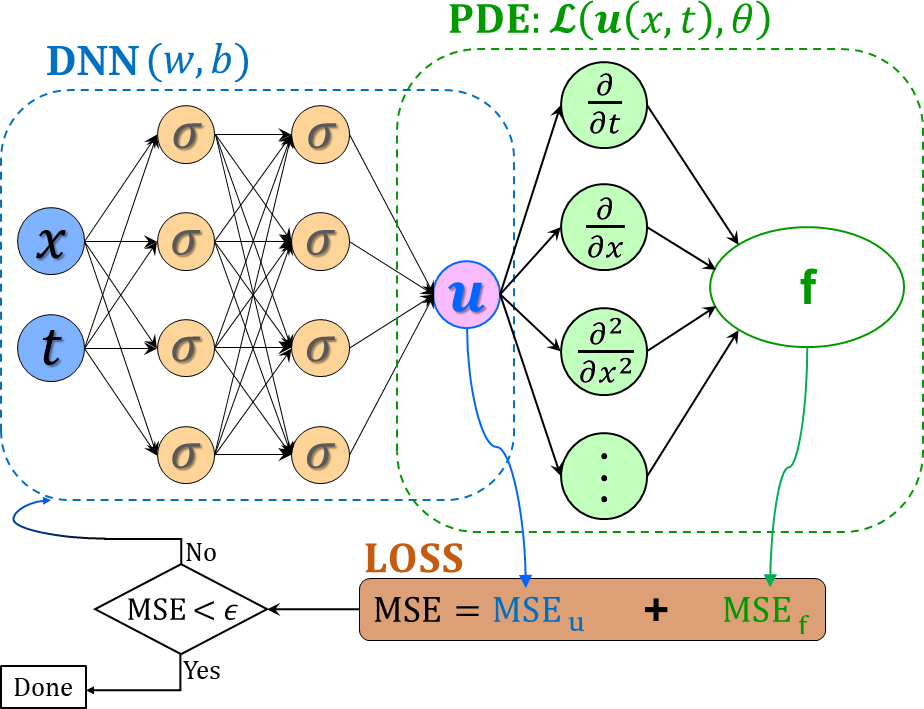
\includegraphics[width=.8\columnwidth]{nn}
\caption{Schematic showing an example structure and loss function, for the PINN approach. The symbol $\theta$ represents the optimization algorithm. The $\epsilon$ represents the smallest threshold error in the optimization algorithm.\\
Source: Adapted from \citeonline{Meng2020}.}
\label{fig:nn}
\end{figure}

According to the work of \citeonline{Raissi2019}, the standard division of the CP dataset into training, validation and testing is not used in this specific PINN model. Instead, a random sample of CPs from the dataset is taken and used to train the PINN. During training, a specific validation set is not used. After training, the network is used to generate two results: ($i$) the discovery of the PDE parameters, and ($ii$) a prediction of the PDE solution.

Once the parameters have been discovered, in a second step, the resulting PINN model is used to predict the velocity field for all points in the defined space and time domain. This predicted velocity field can then be compared with the exact velocity field (generated by GQM), using a relative error to evaluate the accuracy of the prediction, as suggested in Xu et al. (2022) \cite{Xu2022}. Such a relative error is defined by \autoref{eq:error}.

\begin{equation}
R_{L2} = \frac{\| \widehat{U} - U \|}{\|U\|}
\label{eq:error}
\end{equation}

The $\|U\|$ represents the Euclidean L2 norm, which is given by the Euclidean distance from the vector coordinate to the origin of the vector space, i.e. it is the square root of the sum of the squared components of the vector. In the one-dimensional case, the L2 norm is simply given by the value of the velocity.
The $\| \widehat{U} - {U} \| $ represents the application of the L2 norm to the deviation of the estimated velocity field $\widehat{U}$, with respect to the exact velocity field $U$, considering all dataset points in the space and time domains.

The PINN hyperparameters, like the number of hidden layers $N_l(l = 1, 2, ...)$, and the number of neurons in each layer $N_{le}(e = 1, 2, ...)$, can also be optimized by numerical experimentation (trial and error). Optimization of $N_l$ and $N_{le}$, and eventually of other hyperparameters not employed here, is still an unsolved problem, being made empirically \cite{Xu2022}.

As any neural network, PINNs are subjected to overfitting or underfitting. Overfitting means that the DNN performs very well using the training set, but lacks performance using different, new input data of the test set, i.e. it does not generalize. On the other hand, underfitting means that the model performs poorly on both the training and test sets. Obviously, both overfitting and underfitting imply in poor performance of the neural network \cite{Koehrsen2018}.

%========================================
\subsection{NM-based Parameter Discovery}
\label{sec:npd}
%========================================

The inverse problem solved by the implemented PINN to find the coefficients of the differential operators is then compared to the chosen NM-based method, the Sparse Identification of Nonlinear Dynamical Systems (SINDy) method \cite{Boninsegna2018}. This is a method developed for solving the identification problem of dynamical systems, which are systems that change over time. SINDy uses sparse regression to create a linear combination of basis functions to captures the dynamic behavior of the considered physical system. It employs observational or synthetic data to obtain the governing equations that fit such data of the dynamical systems. The discovered equations can then be used to predict future states, inform control inputs, or enable theoretical research using analytical techniques~\cite{Brunton2016}.

Assuming a physical system that evolves in time $t$ and space $x$ defined by a collection of measurements $x(t)\in \mathbb{R}$. Time evolution of $x(t)$ is modeled by SINDy using a nonlinear function $f(x(t))$ (\autoref{eq:sn1}). The vector $x(t)=[x_1(t), x_2(t), \dots x_n(t)]^\top$ represents the state of the physical system at time $t$. The problem solved by SINDy is shown in \autoref{eq:sn2}, where the function $f(x(t))$ is expressed as a matrix $\Theta$ of basis functions applied to the input data $X$, i.e. $\Theta(X)$, which is then multiplied by a matrix $\Xi$ of coefficients that weighs these basis functions. Along the iterations, these coefficients are optimized until achieving convergence by means of an objective function (\autoref{eq:opt}) that assess the correctness of the solution given by [$\Theta(X)\,\Xi$] at a given iteration. It is assumed that $f(x(t))$ is usually sparse in the space of a suitable set of basis functions, i.e. that much of the coefficients of the matrix $\Xi$ are zero. 

\begin{equation}
\frac{d}{dt}x(t) = f(x(t))
\label{eq:sn1}\end{equation}

\begin{equation}
\dot{X} \; = \Theta \,(X)\,\,\Xi
\label{eq:sn2}
\end{equation}

SINDy applies a sparsity-promoting regression (such as LASSO \cite{Tibshirani2011}) to a library of nonlinear candidate functions produced from the measurements, but restricting the number of basis functions to obtain a compact representation of the function and avoid overfitting. SINDy has been effectively used to solve a variety of problems, including linear and nonlinear oscillators, chaotic systems, and fluid dynamics \cite{Brunton2016}. SINDy is implemented by the sparse regression package PySINDy\footnote{\url{http://pysindy.readthedocs.io}} which includes several implementations for the sparse identification method of nonlinear dynamical systems from various authors, being  comprehensive literature reviews available at \cite{DeSilva2020} and \cite{Kaptanoglu2022}. Part of the code implemented in this work was reused and adapted from PySINDy library examples. PySINDy runs on CPU.

This work employs four of these implementations, known as Sparse Regression Optimizers (SRO), which are part of the parameter discovery package and can be selected separately, producing a result for each choice: Sequentially Threshold Least Squares (STLSQ), Orthogonal Least Squares of Forward Regression (FROLS), Sparse Relaxed Regularized Regression (SR3), and Sparse Stepwise Regression (SSR). To keep things simple, we'll treat each of these as a separate NM.

A code snippet of this framework is shown in \autoref{lst:nm}, where \texttt{optimizer} is the chosen optimization method (exemplified in the code as STLSQ), \texttt{SINDy} defines the model, \texttt{fit} discovers the parameters, and \texttt{print} shows the result. 

\begin{minipage}[htb]{\columnwidth}
\begin{lstlisting}[language=Python, label=lst:nm, 
caption={Python code snippet that implements the NM for data-driven PDE parameter discovery. The STLSQ is one of the optimizers in the PySINDy framework.}]
optimizer = ps.STLSQ(threshold=2, alpha=1e-5, normalize_columns=True)
model = ps.SINDy(feature_library=pde_lib,
                 optimizer=optimizer,
                 feature_names=["u"])
model.fit(u, t=dt)
model.print()
\end{lstlisting}
\end{minipage}%

The dataset used by SINDy for each of the 4 optimizers is the same used in the PINN method, but employing the full dataset instead of the set of CPs. Parameter discovery using PINN required training the network with the set of CPs, use of the Burgers' PDE in the loss function, etc. After training, the predicted velocity field in space and time is then compared to the exact field. In the case of SINDy, the complete dataset is used to obtain the parameters, with no further comparison \cite{Brunton2016}. However, parameters discovered by PINN and SINDy are compared in order to evaluate the accuracy of both approaches using the coefficients of the known PDE as reference. Although possible, some optimizations were not made to SINDy in order to obtain better accuracy, being the default settings of the framework used. These possible optimizations can be performed as future work.

Except in the case of SINDy with the SR3 optimizer, the other optimizers employ the objective function that must be minimized, which can be seen in the \autoref{eq:opt}.

\begin{minipage}[htb]{.95\columnwidth}\bigskip\begin{equation}
\| \ y \ - \ X \ w \ \|^2 \ \ + \ \ \alpha \ \| \ w \ \|^2
\label{eq:opt}\end{equation}
Above, $w$ is the weight matrix containing the set of basis functions that maps the dataset contained in $X$ to the solution $y$, i.e. $w$ corresponds to the 2nd member ([$\Theta(X)\,\Xi$]) of \autoref{eq:sn2}, and $\alpha$ is a regularization coefficient applied to $w$, helping prevent overfitting.
\bigskip\end{minipage}%

In order to minimize the objective function, the STLSQ \cite{Brunton2016} algorithm uses ridge regression with sequential threshold, and iteratively runs the least squares algorithm, but masking elements below a specific threshold. The FROLS \cite{Billings2013} algorithm is a greedy algorithm that iteratively selects the most correlated function in the library. The SSR \cite{Boninsegna2018} is also a greedy algorithm that iteratively eliminates the smallest coefficients. A greedy algorithm is any algorithm that uses the heuristic of choosing the locally optimal solution at every iteration \cite{Black2005}. Regardless of not assuredly finding a global optimal solution, greedy heuristics can produce locally optimal solutions that approximate a globally optimal solution in a reasonable amount of time. Along the iterations, the SSR and FROLS algorithms respectively truncate (or add) one nonzero coefficient at each algorithm iteration.

The SR3 algorithm \cite{Champion2019} is a relaxed and sparse regularized regression with linear (dis)equality constraints that attempts to minimize the objective function (\autoref{eq:sr3}).

\begin{minipage}[htb]{.95\columnwidth}\bigskip\begin{equation}\begin{aligned}
&0.5  \|  y  -  X  w \|^2 + \lambda  R(u) + (0.5 / \nu)  \|  w  -  u  \|^2\\
&\text{subject to } Cw = d
\label{eq:sr3}\end{aligned}\end{equation}
over $u$ and $w$, where $R(u)$ is a regularization function, $C$ is a constraint matrix, and $d$ is a vector of values.
\bigskip\end{minipage}%


%========================================
\section{DNN Preliminary Approach for ecRad}
\label{sec:mcw}
%========================================

The problem requires the emulation, using DNN, of the gas-optical algorithm solution of a modern radiation scheme (RTE+RRTMGP), for a wide range of atmospheric conditions, with errors in the heating rates and top-of-atmosphere radiative forcing, typically below $0.1 K day^{-1}$ and $0.5 W m^{-2}$ \cite{Ukkonen2020}.
What is written below is an explanation more linked to the numerical model, but which serves as a basis for emulation. 

Unlike many other phenomena specified in dynamical models, such as clouds and convection, atmospheric radiative transfer is a well-studied issue that can be correctly represented. Modern radiation codes typically use the correlated k approximation and the k-distribution approach to handle the complexity \cite{Goody1989}. The highly variable absorption coefficient spectrum as a function of wavelength, k($\lambda$), is rearranged by $k$ and replaced with a monotonically increasing function $k(g)$, where $g(k)$ is the cumulative distribution function. This function is integrated using a restricted number of quadrature points, referred to as $g$ points. Compared to the line-by-line method, this method significantly reduces the number of monochromatic calculations needed to retrieve fluxes in the SW and LW spectra. 

K-distributions can be applied to an inhomogeneous medium, such as the atmosphere, providing that the mapping of wavelengths to g-space is completely correlated for neighboring atmospheric layers, an approximation that allows fluxes and heating rates to be estimated with less than 1\% uncertainty \cite{Fu1992}. Despite the effectiveness of the correlated k-distribution (CKD) method, radiation calculations in climate models are expensive and performed on a coarser horizontal and temporal grid than others. The ECMWF high-resolution forecast model calls the radiation scheme every 1 hour on a grid with 10.24 times fewer columns than the rest of the model \cite{Hogan2018}.

Because radiation calculations in climate models are expensive, they appear to be a viable area of study for optimizing efficiency without losing accuracy, and one possible approach is the use of PIML.
An interesting aspect about PIML that can be explored in research is the increase in performance of algorithms through the use of single-precision floating-point numbers and the GPU, which is a known feature in algorithms that use DNN.
The preliminary work shows a DNN implementation replacing an existing numerical implementation of the gas-optical scheme (from RRTMGP) of the eCrad model, where performance gains were obtained in preliminary tests, paving the way for future work and a proposal for investigation and implementation of PIML.


%========================================
\subsection{DNN-based Gas Optics Implementation}
\label{sec:mgom}
%========================================

As previously mentioned, the thesis proposes a PIML-based implementation to replace the numerical radiation module ecRad employed in the IFS model of the ECMWF. However, as a preliminary work, a DNN-based model of the RRTMGP gas-optical scheme was implemented for a test case involving a reduced database. The RRTMGP numerical code is part of ecRad module. The accuracy and performance of the DNN implementation were analyzed, taking as reference the corresponding numerical implementation RRTMGP.

The DNN implementation of the gas-optical scheme of the radiation module shown here, the original numerical code (RRTMGP) was replaced by a DNN model. The kernel of the original RRTMGP scheme was written in Fortran 90, and performs a 3D linear interpolation of the optical depth of the atmosphere for the considered 2D grid point using a lookup table indexing temperatures, pressures and mixing fractions. RRTMGP stand for Rapid Radiative Transfer Model for General circulation model (GCM) applications – Parallel \cite{Pincus2019}. It is based on RRTM-G, the Rapid Radiative Transfer Model for GCM-Parallel applications \cite{Hogan2017}. This is a free and open source package that predicts the optical properties of the gaseous atmosphere, includes the solver of the Radiative Transfer Equation called Radiative Transfer for Energetics (RTE), and is used in (numerical) climate and weather models \cite{Pincus2019}. This scheme, like others, includes SW (shortwave) solar radiation and LW (longwave) thermal radiation solving. It employs a statistical k-distribution model based on advanced spectroscopy and numerous g-points, with 256 within 16 LW bands and 224 within 14 SW bands. The RRTMGP code implemented in this work was adapted from \citeonline{Ukkonen2023}. 

The DNN implementation of the gas-optical scheme was developed in a framework composed of the Python 3.12 and the TensorFlow 2.16 library in order to perform training and validation of a MLP neural network using a known dataset. The resulting trained model is saved to disk to later be used in the DNN implementation in Fortran 90 inserted in the radiation module. This Fortran 90 code can be run on CPU or GPUs using cuBLAS and OpenACC, while TensorFlow uses GPU. In the ecRad radiation module, the DNN code is based on Neural Fortran, being called RRTMGP-NN \citeonline{Curcic2019}. 

The standalone ("offline") version of ecRad used in this work is modular, runs on a Unix-like platform, operates independently, and allows investigations and research related to cloud radiative effects without being tied to the operational forecasting model.  It has four components: Gas Optics, Aerosol Optics, Cloud Optics, and Solver. ecRad offers several solvers, including McICA (Monte-Carlo Independent Column Approximation), Tripleclouds, and SPARTACUS \cite{Ukkonen2023}. There is a test version for practical test cases that may run on a standard laptop with GPU and minimum RAM, which was employed in this work and had its performance evaluation analyzed with the Gprof tool.

The input data to the DNN are the temperature, pressure and concentrations of each gas represented in the RRTMGP and, excluding oxygen and nitrogen which are assumed to be constant, this results in 18 LW and 7 SW inputs. In order to predict absorption and Rayleigh optical depths in SW and Planck and absorption optical depths in LW, different models are trained. These are multi-output DNNs that predict all g-points simultaneously, with output sizes of 256 LW or 224 SW. 
In the main code, written in Fortran, the originally numerical gas-optical implementation is replaced by the DNN implementation, also written in Fortran, which uses trained models saved on disk.
The training of the DNN network to obtain the prediction model is implemented in Python using the TensorFlow library, and the final trained model is saved to disk for later use by the Fortran implementation of the main code.
The MLP architectures (layers and neurons) that were used, are described in \autoref{tab:nnmodel}.
In the implementation of the DNN network used in this work, a manual adjustment of the architecture was made, however it would be interesting to use an automated method in future work.
One point that is particularly interesting for the study is that identifying an effective loss function is a significant task, since decreasing the instantaneous imprecision of a specific variable does not guarantee numerical stability over long time intervals, realistic variability, or conservation of energy, moisture, and momentum.

\begin{table}[htb]\centering
\begin{tabular}{cccc}
\hline
     Predicted & Input & 2 Layers & Output \\
\hline
     LW absorption & 18 & 58-58 & 256 \\
     LW emission & 18 & 16-16 & 256 \\
     SW absorption & 7 & 48-48 & 224 \\
     SW scattering & 7 & 16-16 & 224 \\
\hline
\end{tabular}
\vspace{1em}
\caption{Network architectures used for different optical depths.\\
Source: Adapted from \citeonline{Ukkonen2020}.}
\label{tab:nnmodel}
\end{table}

The underlying data flow in a framework of a conventional numerical gas-optical scheme (e.g., RRTMGP) is shown in \autoref{fig:lookup-01}, and the gas-optical scheme it emulates is shown in  \autoref{fig:lookup-02}. In the numerical model, the code calculates the absorption by 1 to 2 major gas species by 3D interpolation in temperature, pressure, and the relative abundance ($\eta$) \cite{Pincus2019}, and contributions from less important gases are computed separately using 2D interpolation, with a given band being written multiple times. In the case of DNN gas optics, all spectral points are predicted simultaneously from an input matrix that includes all gases.

\begin{figure}[htb]\centering
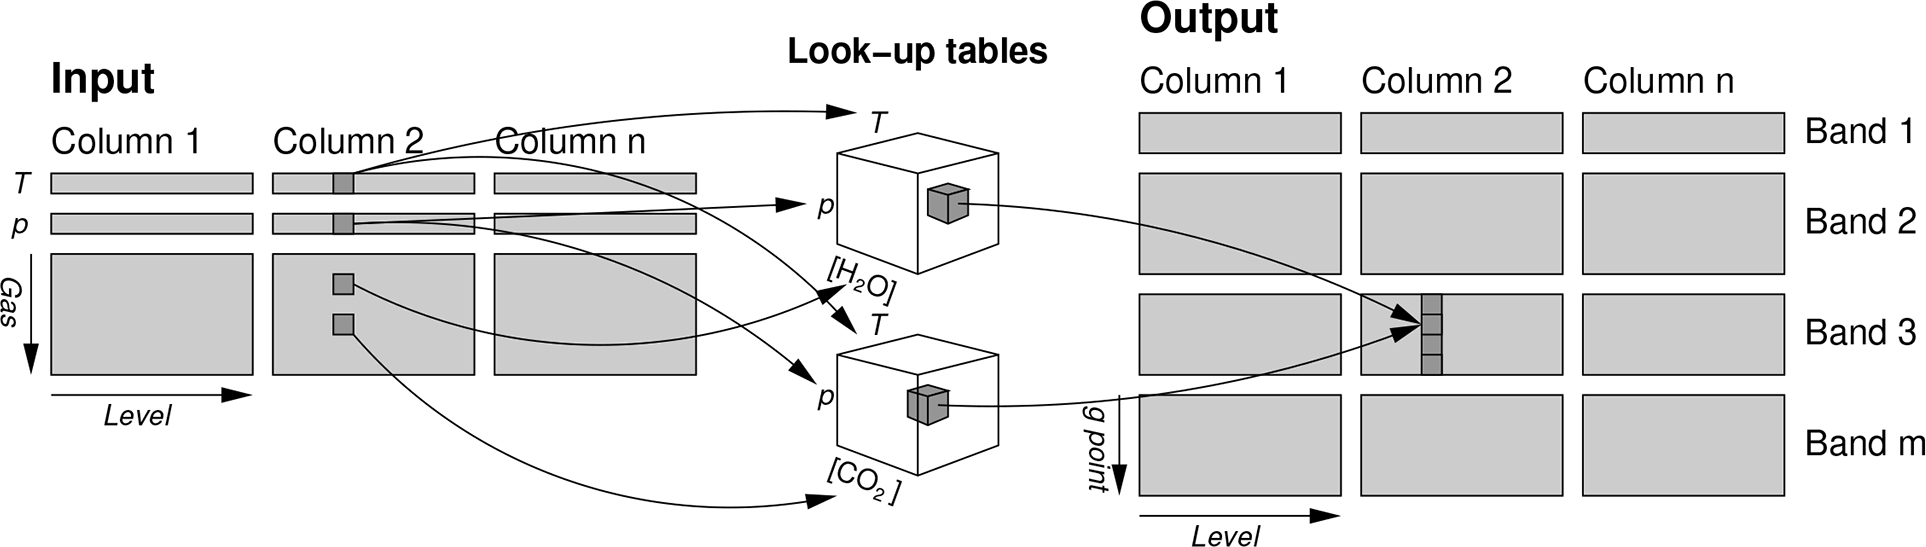
\includegraphics[width=\columnwidth]{lookup-01.png}
\caption{Schematic illustrating the data flow in a structure of a conventional numeric gas optics scheme. "T" is temperature, "p" is pressure, "Gas" represents relative abundance, "Band" corresponds to the LW and SW radiation bands, "g-points" correspond to "k-terms" of the correlated k-distribution method, “Level” corresponds to atmospheric layers or vertical grid points within a column representing altitude or pressure, and "look-up tables" (LUT) correspond to the look-up table kernels of the RRTMGP model. The \autoref{fig:lookup-02} complements this Figure.\\
Source: Adapted from \citeonline{Ukkonen2023}.}
\label{fig:lookup-01}
\end{figure}

\begin{figure}[htb]\centering
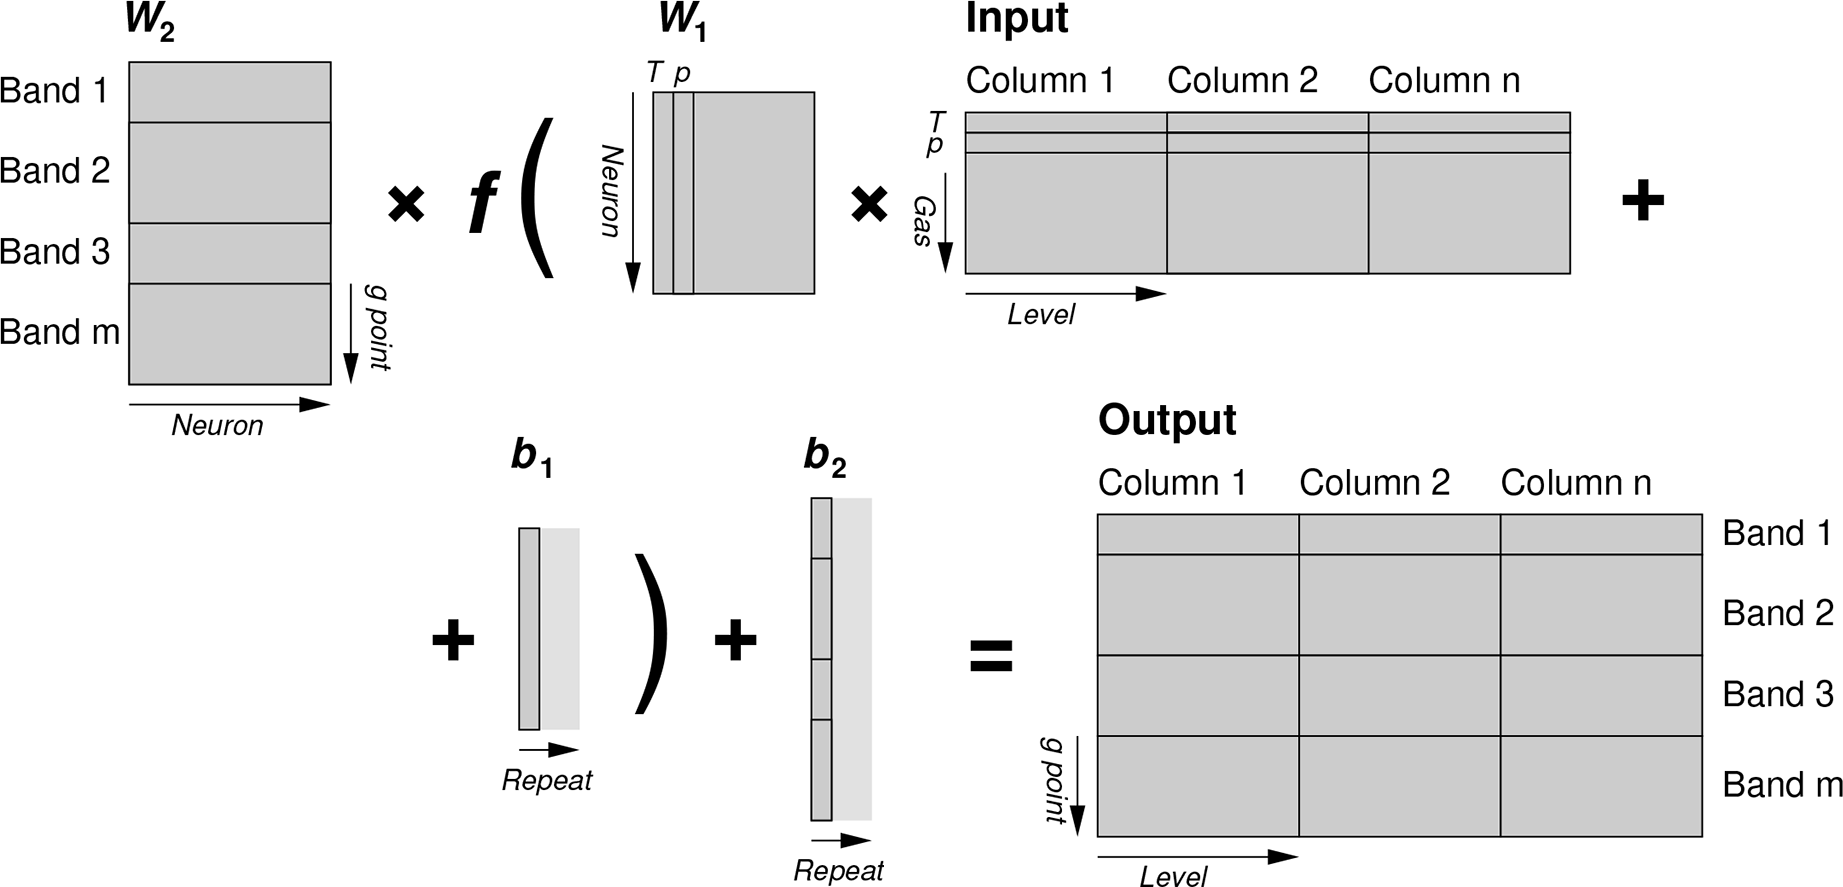
\includegraphics[width=\columnwidth]{lookup-02.png}
\caption{Simplified schematic, with only one hidden layer, illustrating the data flow in a gas optics DNN framework. "W" represents weight, and "b" represents bias. The other terms are described in the \autoref{fig:lookup-01}.\\
Source: Adapted from \citeonline{Ukkonen2023}.}
\label{fig:lookup-02}
\end{figure}

For a given band, vertical level, and column, the RRTMGP calls interpolation kernels several times to compute gas-specific contributions to optical properties, accounting for temperature (T) and pressure (p) dependencies, as well as overlap of major gases in the band. These kernels loop over the g points in a single band, of which there are only 1-12 in the reduced k distributions.

The DNN improves performance by (i) predicting a vector containing all g points from a vector containing T, p, and the mixing ratios of all gases (the DNN implicitly treats gas interactions) and (ii) batching the computations for multiple atmospheric levels and columns by expressing the core DNN computations as matrix-matrix multiplications (between weights W and input matrices) that are delegated to a BLAS library. 

In the chosen DNN loss function (\autoref{eq:ecrnn}), $\alpha$ is a coefficient representing a trade-off between heating rate and radiative forcing errors (e.g. 0.6 for LW and 0.2 for SW), $y$ is the target vector, and $\hat{y}$ is the DNN output vector. It minimizes the error in the difference in y associated with different perturbation experiments as well as the mean squared error of y (scaled DNN outputs) and indirectly measures radiative forcing errors.

\begin{equation}
loss = \alpha \sum_{i=1}^{N}(y_i - \hat{y}_i)^2 + (1 - \alpha)
\sum_{\substack{i=1 \\ i \ \text{odd}}}^{N} ( (y_{i+1} - y_i) - (\hat{y}_{i+1}-\hat{y}_i) )^2
\label{eq:ecrnn}
\end{equation}

The training dataset used is derived from a variety of sources, including existing atmospheric profiles, future climate experiments, and reanalyses, which were synthetically supplemented by varying greenhouse gas concentrations, either manually or using hypercube sampling, as well as data provided by the Radiative Forcing Model Intercomparison Project \cite{Pincus2016}, which includes 100 profiles and 18 perturbations. The profiles were designed to assess global mean clear-sky errors in instantaneous radiative forcing and should be well suited as an out-of-sample test for our purposes, and in addition, a different dataset based on the CAMS reanalysis \cite{Inness2019} is also used that uses the same approach as the IFS and the Correlated k-distribution Model Intercomparison Project (CKDMIP) \cite{Hogan2020}, where only nine gases are considered, but the radiative forcing.

For performance analysis, Gprof was used, which is a performance analysis tool for Unix-based programs, developed as an expanded version of the previous "prof" tool, using a combination of instrumentation and sampling, and which can collect and print a limited number of call graphs. Two analyses were performed, one of the original numerical implementation of ecRad, and another of the version that uses the DNN implementation. The goal was to identify, in a general way, without going into too much detail, the main costly routines.


%========================================
\section{Computing Environment}
\label{sec:cenv}
%========================================

The DNN, PINN and the four PySINDy codes\footnote{The codes are available at \url{http://github.com/efurlanm/pd1b24}} were executed in three different computing environments. It is important to note that the PINN model runs on GPU, DNN runs on CPU/GPU, and PySINDy runs on CPU. The first environment (used in 1D Burgers') is a PC with a 6-core Intel i7-9750H CPU with 6 cores, 8 GB of main memory, and an NVIDIA GTX 1050 GPU (768 CUDA cores and 3 GB of memory). The second (used in DNN RRTMGP) is a PC with 2-core Intel I7-7500U CPU with 2 cores, 16 GB of main memory, and an NVIDIA Geforce 940MX GPU (384 CUDA cores and 4 GB of memory). The third environment (used in DNN RRTMGP) is the Santos Dumont (SDumont) supercomputer of the National Scientific Computing Laboratory (LNCC), more specifically a single Bull Sequana X1120 processing node with two 24-core Intel Xeon Gold 6252 Skylake 2.1 GHz processors (total of 48 cores), 384 GB of main memory and four Nvidia Volta V100 GPUs, although only one GPU was employed. Both computing environments included the Python\footnote{\url{http://www.python.org}} 3.7 interpreter and the TensorFlow\footnote{\url{http://www.tensorflow.org}} v1.15 machine learning platform.

 %% 2o capítulo
%========================================
\chapter{RESULTS}
\label{ch:resu}
%========================================

Results are presented in this chapter for the previous work, application of a PINN implementation for the 1D Burgers equation, and the current preliminary work, the DNN-based gas optics implementation.


%========================================
\section{PINN Implementation for the 1D Burgers Equation}
%========================================

The results for the 1D Burger's equation are divided into two parts of experiments: 
(i) the first compares the results of PINN with the 4 SINDy versions; 
(ii) the second evaluates the PINN implementation for various hyperparameters and CP sizes.

The first part uses datasets related to different problem sizes ($x$ space versus $t$ time discretization): 128x64, 256x128, and 512x256, while the second part uses only a 256x100 problem size. The GQM is used to generate the dataset corresponding to the exact solution (reference), which are then employed by the SINDy versions, and also to extract the set of CPs used by the PINN implementation. The MLP architecture used for the PINN implementation in the first part has one input layer, 3 hidden layers with 20 neurons each, and one output layer. The PINN undergoes training and PDE parameters are estimated, solving the inverse problem, and the resulting model estimates the solution (space versus time field). The processing-time data obtained in the all experiments is given by the average of 3 executions. 

%========================================
\subsection{Comparison of PINN and SINDy parameter discovery}
%========================================

Tables \ref{tab:nm-pinn-time-comp-01} and \ref{tab:nm-pinn-time-comp-02} show  the average of elapsed times of 3 runs on the local machine for the PINN (using GPU) and the 4 SINDy implementations (only CPU), for the 3 problem sizes and for the two cases of viscosity.  In the case of PINN, training time to estimate the parameters and prediction time of the resulting 1D field using the trained model are shown. Processing times of SINDy versions are consistently lower than those of the PINN model, even considering that the latter executes using GPU. Therefore, future studies must consider the tradeoff between accuracy and processing times when comparing PINNs and numerical methods like SINDy. 

\begin{table}[htb]\centering
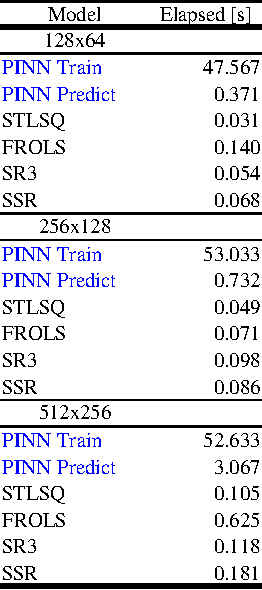
\includegraphics[width=.27\columnwidth]{nm-pinn-time-comp-01}
\vspace{1em}
\caption{Comparison of elapsed times (average of 3 runs) for the PINN and the 4 SINDy models for kinematic viscosity of the fluid of ${0.01}/{\pi}$, and for execution on the local machine (PC).}
\label{tab:nm-pinn-time-comp-01}
\end{table}

\begin{table}[htb]\centering
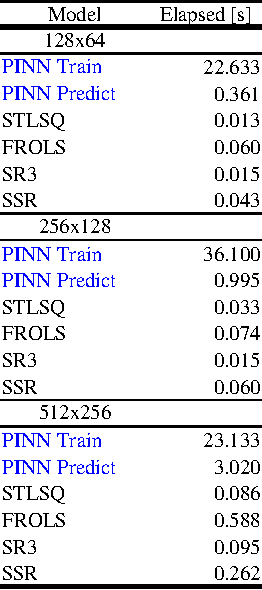
\includegraphics[width=.27\columnwidth]{nm-pinn-time-comp-02}
\vspace{1em}
\caption{Comparison of elapsed times (average of 3 runs) for the PINN and the 4 SINDy models for kinematic viscosity of the fluid of ${0.1}/{\pi}$, and for execution on the local machine (PC).}
\label{tab:nm-pinn-time-comp-02}
\end{table}

Tables \ref{tab:nm-pinn-01} and \ref{tab:nm-pinn-02} show the results obtained for the PDE parameter discovery, comparing the  PINN and the 4 SINDy implementations (STLSQ, FROLS, SR3 and SSR, discussed in \autoref{sec:npd}), and also considering 2 different viscosity values in the 1D Burgers' equation, ${0.01}/{\pi}$ and ${0.1}/{\pi}$. As already commented, 3 sizes of problems are considered: 128x64, 256x128 and 512x256. 

Subscripts denote partial differentiation in time and space, e.g. u\_x denotes ${du}/{dx}$, u\_xx denotes ${d^2u}/{dx^2}$, and so on. -At the top of each table is shown the \textit{Exact PDE} 1D Burgers' equation (e.g., $u_t + 1.0 u u_x - 0.003183 u_{xx} = 0$) used to generate the datasets.

In the case of PINN, training is done using 2,000 CPs randomly obtained from the dataset, regardless of the size of the problem.  In the case of SINDy implementations, the complete dataset is used in the model to obtain the parameters. In \ref{tab:nm-pinn-01} the viscosity value (${0.01}/{\pi}$) is lower than in the second (${0.1}/{\pi}$) in order to check if SINDy accuracy is compromised for  small viscosity values, as confirmed by the results. PINN accuracy was good, even using the set of CPs extracted from the smaller dataset, and such accuracy improves with the problem size. \ref{tab:nm-pinn-01} is for experiments with the higher viscosity value, showing that the accuracy of the SINDy implementations improved in comparison to the results of the preceding table, but are still lower than those obtained by PINN.

\begin{table}[htb]\centering
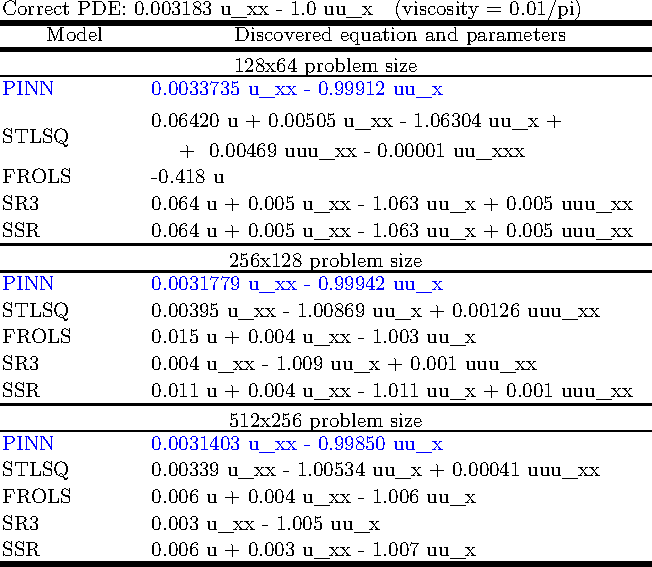
\includegraphics[width=.7\columnwidth]{nm-pinn-01}
\vspace{1em}
\caption{Comparison of the results of the parameter discovery for the 1D Burgers' equation using PINN (in blue) and the 4 SINDy versions (kinematic viscosity of the fluid of ${0.01}/{\pi}$).}
\label{tab:nm-pinn-01}
\end{table}

\begin{table}[htb]\centering
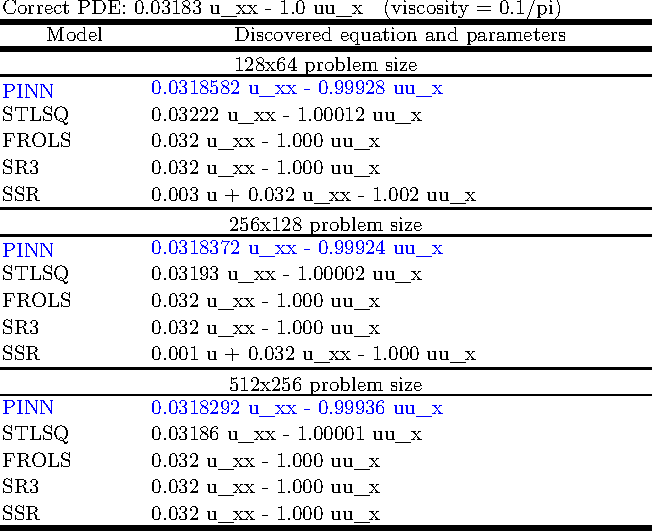
\includegraphics[width=.7\columnwidth]{nm-pinn-02}
\vspace{1em}
\caption{Comparison of the results of the parameter discovery for the 1D Burgers' equation using PINN (in blue) and the 4 SINDy versions (kinematic viscosity of the fluid of ${0.1}/{\pi}$).}
\label{tab:nm-pinn-02}
\end{table}

The next subsections present the solution field $u(t,x)$ generated by the PINN implementation for the 3 problem sizes, and for the 2 viscosity values. For each case, there are figures showing the predicted solution $u(t,x)$ with marks representing the CPs, and a particular snapshot at time $t=0.5$ comparing the PINN prediction and the exact solution. These figures allow a visual assessment of the accuracy of the solutions.

\FloatBarrier

%========================================
\subsubsection{Problem Size 128x64}
%========================================

Figures \ref{fig:pinn-01-128-a}, \ref{fig:pinn-01-128-b}, \ref{fig:pinn-02-128-a}, and \ref{fig:pinn-02-128-b} show, for the problem size 128x64, the solutions for the viscosities ${0.01}/{\pi}$ and ${0.1}/{\pi}$. Figures \ref{fig:pinn-01-128-a} and \ref{fig:pinn-02-128-a} show the predicted spatio-temporal solution $u(t, x)$, and the CPs used to training are represented as dark marks on the graph. Since the dataset is relatively small and the number of CP is 2,000, the small marks are aligned and may not appear random at first. 
At the top and bottom of the figure, ($x=1.0$ and $x=-1.0$), are the CPs related to the boundary conditions (BC) of the PDE, on the left side ($t=0, 0$) are the CPs relative to the initial conditions (IC), and in the center of the figure ($x=0.0$) the complex non-linear behavior (sometimes called formation of a shock wave) of the Burgers' equation with lower viscosity is represented. The remaining randomly selected CPs appear on the graph. Although it was not done this way, it is possible to select more points in the BC and IC regions to reinforce network training, if necessary.

Figures \ref{fig:pinn-01-128-b} and \ref{fig:pinn-02-128-b} show a snapshot in time comparing the superimposed solution for the PINN method and the exact numerical solution.
It is possible to see that even using a few CPs, the PINN was able to accurately capture the complex non-linear behavior of the Burgers' equation, which presents the formation of an accentuated internal layer around t = 0.4, which is generally difficult to solve with traditional NM and requires a laborious spatio-temporal discretization of the equation. 
In this scenario, we can directly address the nonlinear problem without needing to commit to any prior assumptions, linearization, or local time step.

\begin{figure}[htb]\begin{minipage}[b]{\textwidth}\centering
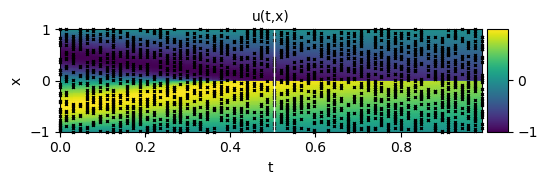
\includegraphics[width=.75\columnwidth]{pinn-01-128-a}
\vspace{-1em}
\caption{PINN predicted solution $u(t, x)$ for viscosity ${0.01}/{\pi}$ and problem size 128x64.}
\label{fig:pinn-01-128-a}
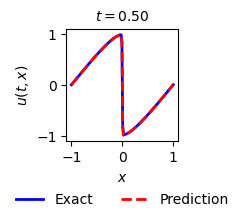
\includegraphics[width=.4\columnwidth]{pinn-01-128-b}
\vspace{-1em}
\caption{Comparison of the solutions obtained by PINN (in red) and the exact numerical solution (in blue) for the $t=0.5$ snapshot (viscosity of ${0.01}/{\pi}$ and problem size of 128x64).}
\label{fig:pinn-01-128-b}
\end{minipage}\end{figure}

\begin{figure}[htb]\begin{minipage}[b]{\textwidth}\centering
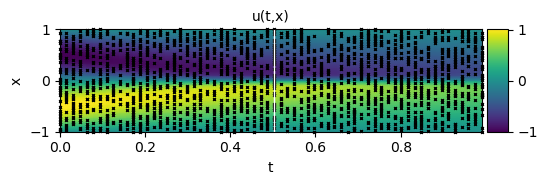
\includegraphics[width=.75\columnwidth]{pinn-02-128-a}
\vspace{-1em}
\caption{PINN predicted solution $u(t, x)$ for viscosity ${0.1}/{\pi}$ and problem size 128x64.}
\label{fig:pinn-02-128-a}
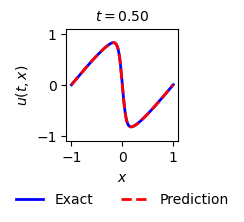
\includegraphics[width=.4\columnwidth]{pinn-02-128-b}
\vspace{-1em}
\caption{Comparison of the solutions obtained by PINN (in red) and the exact numerical solution (in blue) for the $t=0.5$ snapshot (viscosity of ${0.1}/{\pi}$ and problem size of 128x64).}
\label{fig:pinn-02-128-b}
\end{minipage}\end{figure}

Due to the number of CPs being constant even when the size of the dataset varies, great variation in the discovery of parameters in the PINN model is not expected. In the case of the NMs seen in Tables \ref{tab:nm-pinn-01} and \ref {tab:nm-pinn-02}, the variation is expected because the NM uses the complete dataset (does not use CP). In addition, there is also variation related to each NM algorithm. For the \autoref{tab:nm-pinn-01} with lower viscosity, it is possible to observe that for 128x64 (total of 8,192 data points) the accuracy of the NM was not good, unlike the PINN model which obtained good accuracy even with a smaller amount (2000 CPs) of training data. As for \autoref{tab:nm-pinn-02} with higher viscosity, it is possible to observe that for 128x64 the NM showed better accuracy, especially FROLS and SR3, approaching the PINN model.

\FloatBarrier

%========================================
\subsubsection{Problem Size 256x128}
%========================================

The Figures \ref{fig:pinn-01-256-a}, \ref{fig:pinn-01-256-b}, \ref{fig:pinn-02-256-a} and \ref{fig:pinn-02-256-b} show, for the problem size 256x128, the solutions for the viscosities ${0.01}/{\pi}$ and ${0.1}/{\pi}$. Much of what was presented in the previous section also applies to this section. In Figures \ref{fig:pinn-01-256-a} and \ref{fig:pinn-02-256-a} one can initially observe a better distribution of CPs in a more random way, due to the fact that the set of data to be larger and the size of the CP set remains at 2,000 CPs, allowing the CP to be distributed a little better in the graph. Figures \ref{fig:pinn-01-256-b} and \ref{fig:pinn-02-256-b} show the same behavior as the previous subsection, even because the amount of CP is the same. For the \autoref{tab:nm-pinn-01} with lower viscosity, and 256x128 problem size, the NMs were not accurate. For low viscosity, in most cases, regardless of the dataset, the PINN model showed better accuracy. For the \autoref{tab:nm-pinn-02} with higher viscosity, and 256x64 problem size, most of the NMs behaved well, differently from what occurs in the case with lower viscosity.

\begin{figure}[htb]\begin{minipage}[b]{\textwidth}\centering
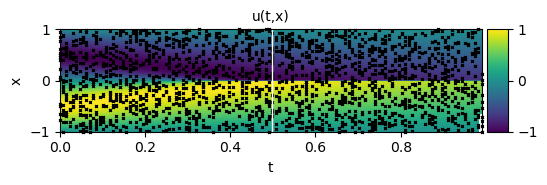
\includegraphics[width=.75\columnwidth]{pinn-01-256-a}
\vspace{-1em}
\caption{PINN predicted solution $u(t, x)$ for viscosity ${0.01}/{\pi}$ and problem size 256x128.}
\label{fig:pinn-01-256-a}
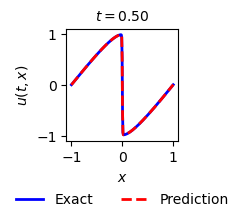
\includegraphics[width=.4\columnwidth]{pinn-01-256-b}
\vspace{-1em}
\caption{Comparison of the solutions obtained by PINN (in red) and the exact numerical solution (in blue) for the $t=0.5$ snapshot (viscosity of ${0.01}/{\pi}$ and problem size of 256x128).}
\label{fig:pinn-01-256-b}
\end{minipage}\end{figure}

\begin{figure}[htb]\begin{minipage}[b]{\textwidth}\centering
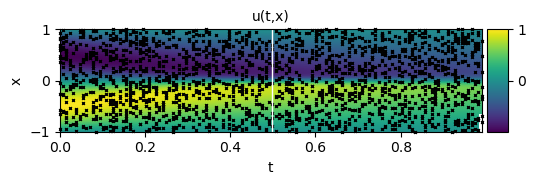
\includegraphics[width=.75\columnwidth]{pinn-02-256-a}
\vspace{-1em}
\caption{PINN predicted solution $u(t, x)$ for viscosity ${0.1}/{\pi}$ and problem size 256x128.}
\label{fig:pinn-02-256-a}
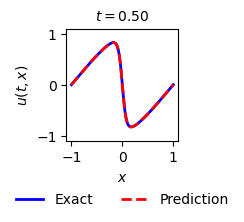
\includegraphics[width=.4\columnwidth]{pinn-02-256-b}
\vspace{-1em}
\caption{Comparison of the solutions obtained by PINN (in red) and the exact numerical solution (in blue) for the $t=0.5$ snapshot (viscosity of ${0.1}/{\pi}$ and problem size of 256x128).}
\label{fig:pinn-02-256-b}
\end{minipage}\end{figure}

%========================================
\subsubsection{Problem Size 512x256}
%========================================

The Figures \ref{fig:pinn-01-512-a}, \ref{fig:pinn-01-512-b}, \ref{fig:pinn-02-512-a} and \ref{fig:pinn-02-512-b} show, for the problem size 512x256, the same behavior as the previous subsection. For Tables \ref{tab:nm-pinn-01} and \ref{tab:nm-pinn-02}, 512x256 problem size, the NMs showed similar behavior to the previous section, with the SSR method standing out.

\begin{figure}[htb]\begin{minipage}[b]{\textwidth}\centering
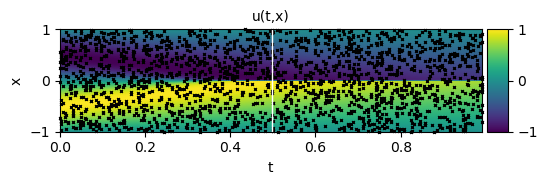
\includegraphics[width=.75\columnwidth]{pinn-01-512-a}
\vspace{-1em}
\caption{PINN predicted solution $u(t, x)$ for viscosity ${0.01}/{\pi}$ and problem size 512x256.}
\label{fig:pinn-01-512-a}
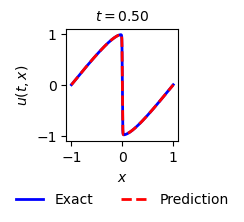
\includegraphics[width=.4\columnwidth]{pinn-01-512-b}
\vspace{-1em}
\caption{Comparison of the solutions obtained by PINN (in red) and the exact numerical solution (in blue) for the $t=0.5$ snapshot (viscosity of ${0.01}/{\pi}$ and problem size of 512x256).}
\label{fig:pinn-01-512-b}
\end{minipage}\end{figure}

\begin{figure}[htb]\begin{minipage}[b]{\textwidth}\centering
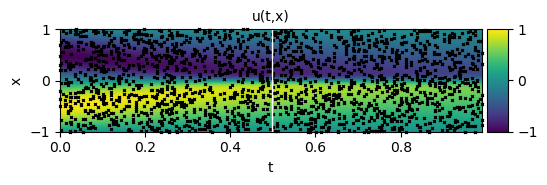
\includegraphics[width=.75\columnwidth]{pinn-02-512-a}
\vspace{-1em}
\caption{PINN predicted solution $u(t, x)$ for viscosity ${0.1}/{\pi}$ and problem size 512x256.}
\label{fig:pinn-02-512-a}
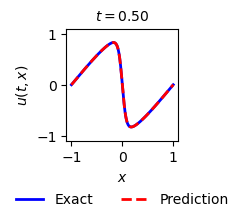
\includegraphics[width=.4\columnwidth]{pinn-02-512-b}
\vspace{-1em}
\caption{Comparison of the solutions obtained by PINN (in red) and the exact numerical solution (in blue) for the $t=0.5$ snapshot (viscosity of ${0.1}/{\pi}$ and problem size of 512x256).}
\label{fig:pinn-02-512-b}
\end{minipage}\end{figure}

\FloatBarrier

%========================================
\subsection{Evaluation of PINN Hyperparameters and CP Size}
%========================================

PINN processing time and accuracy is evaluated using the model generated with different sets of hyperparameters and CP set sizes in experiments executed on SDumont. Resulting predicted 1D fields are presented in figures, which are similar to those of the previous section. Following, PINN accuracy and processing times are evaluated as a function of the number of neurons per hidden layer, the number of hidden layers, and also the size of the CP set.

%========================================
\subsubsection{Visual Assessment of PINN}
%========================================

In this section, the network architecture is the same employed for the preceding comparisons between PINN and SINDy implementations (single input and output layers and 4 hidden layers with 20 neurons each). A visual assessment of predictive accuracy for problem size 256x100 and fluid viscosity of 0.01 is shown in \autoref{fig:bur1}, with time $t$ on the horizontal axis and spatial coordinate $x$ on the vertical axis. The color scale refers to the velocity $u(t, x)$. The black dots on the graph represent the 2,000 CPs randomly generated from the dataset and used for training. The \autoref {fig:bur2} shows a specific snapshot at $t=0.5$, where it is possible to observe the overlapping solutions for PINN and GQM (exact).  For this specific result, the equation obtained by PINN is $u_t + 0.99967 u u_x - 0.0030988 u_{xx} = 0$, while the exact PDE is $u_t + u u_x - 0 ,0031831 u_{xx} = 0$. Thus, the PINN could identify the underlying PDE with good accuracy.

\begin{figure}[htb]\begin{minipage}[b]{\textwidth}\centering
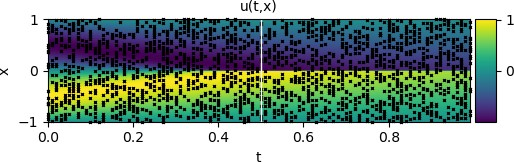
\includegraphics[width=.75\columnwidth]{burg-01.jpg}
\vspace{0em}
\caption{PINN predicted solution $u(t, x)$ for viscosity ${0.01}/{\pi}$ and problem size 256x100 (black dots denote the 2,000 randomly assigned CPs).} 
\label{fig:bur1}
\vspace{1em}
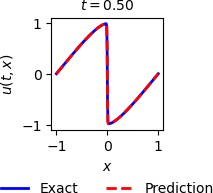
\includegraphics[width=.35\columnwidth]{burg-02.jpg}
\vspace{0em}
\caption{Comparison of the solutions obtained by PINN (in red) and the exact numerical solution (in blue) for the $t=0.5$ snapshot (viscosity of ${0.01}/{\pi}$ and problem size of 256x100).}
\label{fig:bur2}
\end{minipage}\end{figure}

%========================================
\subsubsection{Influence of the Layers and Neurons in the PINN}
%========================================

For the results presented below, the hyperparameters $N_{l}$ (number of hidden layers) and $N_{le}$ (number of neurons per hidden layer) were varied, as well as the number of CPs for training. The \autoref{tab:resu1} shows the relative L2 errors and training times of the PINN, for different hyperparameters used: 10, 15, 20, 25, and 30 neurons per hidden layer, and 1, 2, 4, 6, and 8 hidden layers. The number of CPs was set at 2,000. All values shown here are the average of 3 runs. In this table it is possible to observe that there is a tendency for the best values to be concentrated in the center, probably because there is a problem of underfitting or overfitting in the values at the edges of the table. For future work, it would be interesting to better evaluate this behavior. One of the highlights is that the smallest error is obtained with 6 hidden layers, not 8. In this specific case, increasing the number of layers not only does not increase accuracy, it also worsens performance.

The \autoref{fig:rlaygrapherror2} shows that the error for 1 hidden layer is high compared to the other number of layers. For 2 layers, there is a significant improvement in accuracy. For 4, 6, and 8 the gain in precision is not that great, but the curves are similar and are in the region of greater accuracy, showing that they would be the best choices.

The \autoref{fig:rlaygraptime2} shows, for 4 hidden layers, a tendency to describe a curve that resembles a parabolic, with a minimum processing time of 20 neurons per hidden layer. This is probably due to the problem of underfitting and overfitting occurring at the beginning and at the end of the curve. Once again, for future work, it would be interesting to better evaluate this behavior.

\begin{table}[htb]\centering
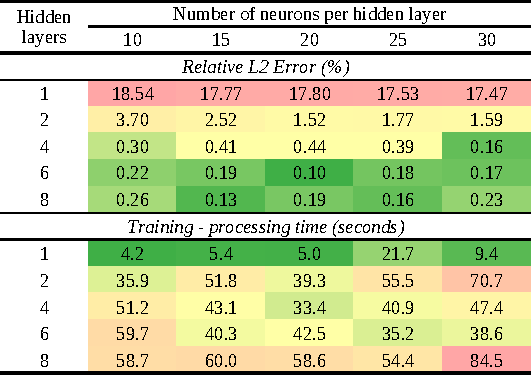
\includegraphics[width=.7\columnwidth]{rlay}
\vspace{1em}
\caption{Relative L2 errors and DNN training times for different number of neurons and hidden layers. On the color scale, the best values are highlighted in green. The simulation ran on the SDumont.}
\label{tab:resu1}
\end{table}

\begin{figure}[htb]\centering
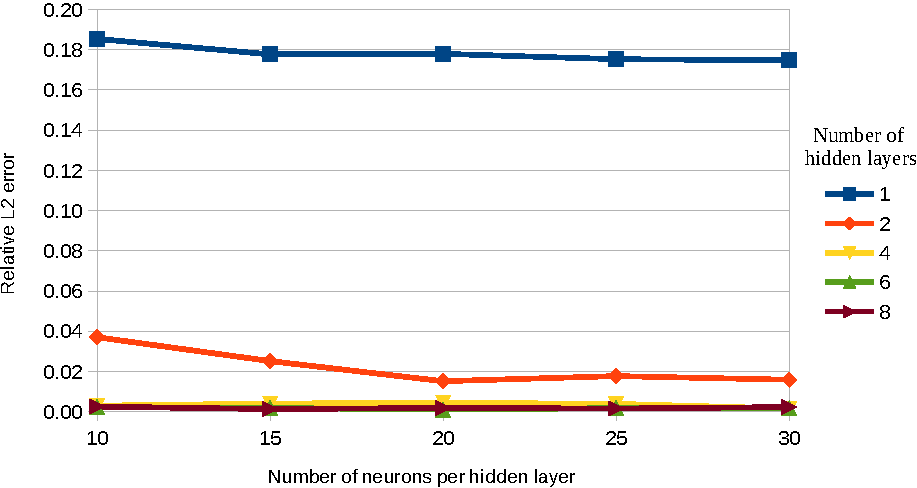
\includegraphics[width=.8\columnwidth]{rlaygrapherror2}
\vspace{0em}
\caption{Relative L2 error (\%) in function of number of neurons and hidden layers. The simulation ran on the SDumont.}
\label{fig:rlaygrapherror2}
\end{figure}

\begin{figure}[htb]\centering
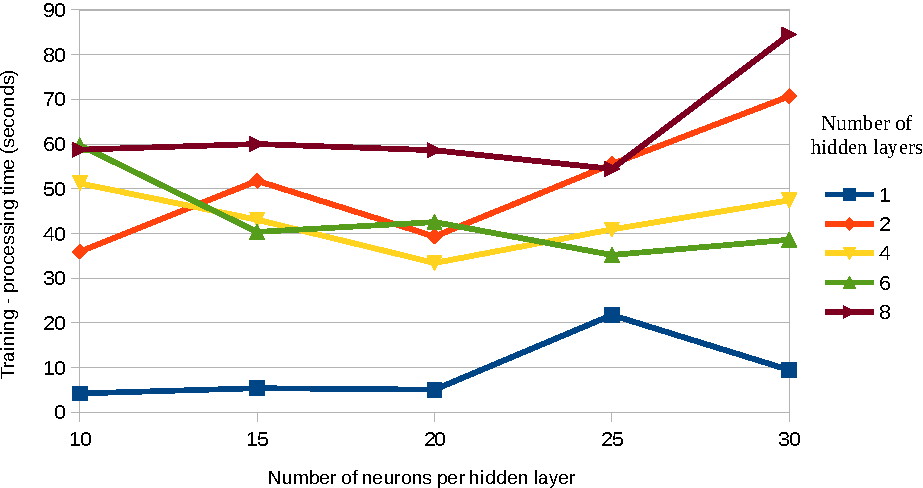
\includegraphics[width=.8\columnwidth]{rlaygraphtime2}
\vspace{0em}
\caption{Processing times (seconds) in function of number of neurons and hidden layers. The simulation ran on the SDumont.}
\label{fig:rlaygraptime2}
\end{figure}

%========================================
\subsubsection{Influence of Neurons and the CP in the PINN}
%========================================

The \autoref{tab:rnu8} shows the relative L2 errors and training times of the PINN, for different hyperparameters and number of CP: 10, 15, 20, 25, and 30 neurons per hidden layer, and 400, 800, 1200, 1600, and 2000 CP. The number of layers was set at 8. All values shown here are the average of 3 runs. In this table, as in the previous one, it is possible to observe that there is a tendency for the best values to be concentrated in the center, probably because the problem of underfitting or overfitting is occurring in the values at the edges of the table. Once again, for future work, it would be interesting to better evaluate this behavior. One of the highlights is that considering the smallest error and the shortest processing time, the best dataset size is 1600, and the best number of neurons per hidden layer is 20.

The \autoref{fig:rnu8graphtime2} shows for most curves a tendency to describe a curve that resembles a parabolic, probably due to the problem of underfitting and overfitting occurring at the beginning and end of the curve. Once again, for future work, it would be interesting to better evaluate this behavior. The shortest processing time occurs for 15 neurons per hidden layer, and 1600 CPs.

The \autoref{fig:rnu8grapherror2} shows that the error for 400 CPs is high compared to the others. 800 CPs presents a significant improvement in accuracy, and the other curves are relatively close, not presenting such a relative large accuracy gain.

\begin{table}[htb]\centering
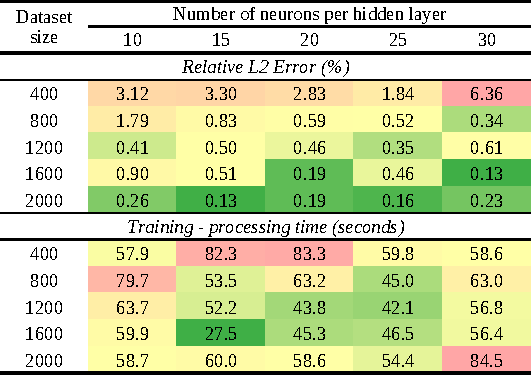
\includegraphics[width=.7\columnwidth]{rnu8}
\vspace{1em}
\caption{Relative L2 errors and DNN training times for different number of neurons and dataset size. The number of hidden layers is set to 8. On the color scale, the best values are highlighted in green. The simulation ran on the SDumont.}
\label{tab:rnu8}
\end{table}

\begin{figure}[htb]\centering
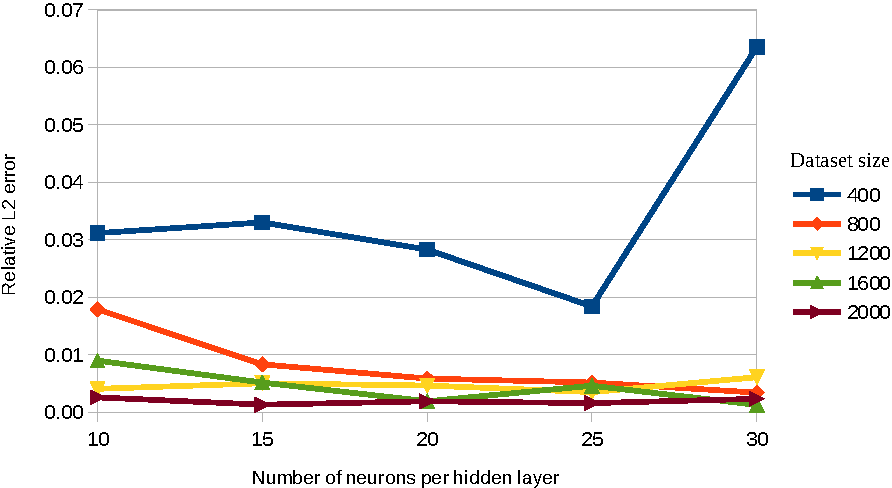
\includegraphics[width=.8\columnwidth]{rnu8grapherror2.pdf}
\vspace{0em}
\caption{Relative L2 error (\%) in function of number of neurons and dataset size. The number of hidden layers is set to 8. The simulation ran on the SDumont.}
\label{fig:rnu8grapherror2}
\end{figure}

\begin{figure}[htb]\centering
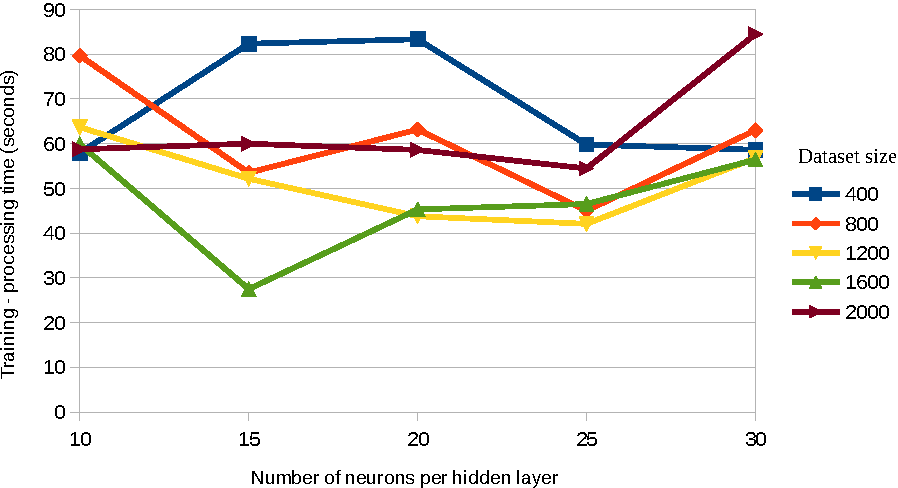
\includegraphics[width=\columnwidth]{rnu8graphtime2.pdf}
\vspace{-1em}
\caption{Processing times (seconds) in function of number of neurons and dataset size. The number of hidden layers is set to 8. The simulation ran on the SDumont.}
\label{fig:rnu8graphtime2}
\end{figure}

%========================================
\subsubsection{PINN Prediction Times}
%========================================

\autoref{tab:rpre} shows the prediction times of the trained PINN model in function of different number of hidden layers (1, 4, 8) and different numbers of neurons per hidden layer (10, 20, 30). As expected, such times are very close, differently from the corresponding training times, which are higher and differ too much. For instance,  in the case of 4 hidden layers and 20 neurons per layer, training time was 33.4 s, while prediction time was only 0.724 s, or 2.2\%. This is a common issue with neural networks, showing the convenience of avoiding re-training the network whenever possible.

\begin{table}[htb]\centering
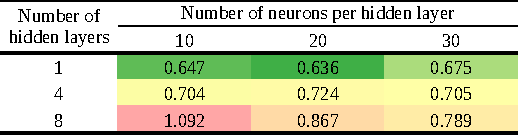
\includegraphics[width=.7\columnwidth]{rpre}
\vspace{1em}
\caption{Prediction times for different number of neurons and hidden layers. On the color scale, the best values are highlighted in green. The simulation ran on the SDumont.}
\label{tab:rpre}
\end{table}






%========================================
%========================================
%========================================
%========================================






\FloatBarrier

%========================================
\section{DNN-Based Gas-Optics Implementation}
\label{sec:resu32}
%========================================

The gas-optical system of the radiation module was implemented using DNN, and the results were compared to those of the implementation using the traditional numerical model. TensorFlow was used to train the DNN, using a dataset derived from various sources. Gprof was used to evaluate the performance of the ecRad versions.


%========================================
%\subsection{DNN-based gas optics model}
%\label{sec:rgom}
%========================================

The result of eCrad running offline with example data is shown in Tables \ref{tab:ecgpr1a} and \ref{tab:ecgpr2a}.
The first table shows the performance analysis of the offline ecRad example with the original numerical scheme, using the gprof tool.
The second table shows the gas-optical DNN version analysis. 
Times are for one run.
The total execution time for the numerical version was 1.55 s, and the time for the DNN version was 1.50 s, showing a performance gain.

\begin{table}[htb]\centering\begin{tabular}{ c c c c c c c } 
\hline
\%	    & cumulative &   self	   &	    &   self	&   total	& \\
time	&  seconds	&  seconds	   & calls	&  ms/call	&  ms/call	& routine \\
\hline
17.42	&      0.27	&     0.27	   & 12	    &    22.50	&    34.06	&  CloudsSW \\
12.90	&      0.47	&     0.20	   & 12	    &    16.67	&    49.17	&  GasOptics \\
12.90	&      0.67	&     0.20	   & 12	    &    16.67	&    30.10	&  CloudsLW \\
9.68	&      0.82	&     0.15	   & 11	    &    13.64	&    13.64	&  Aerosol \\
7.74	&      0.94	&     0.12	   & 4817	&     0.02	&     0.02	&  TransSW \\
\hline \\
\end{tabular}
\caption{The performance analysis using the gprof tool of the offline ecRad example with the original numerical gas-optical scheme. The "routine" column is described in the \autoref{tab:ecgpr1b}. The remaining columns are the standard output of gprof. The total execution time is 1.55 s. Times are for one run.}
\label{tab:ecgpr1a}
\end{table}

\begin{table}[htb]\centering\begin{tabular}{ c c c c c c c } 
\hline
\%	      & cumulative	&   self	&	        &   self	&   total	& \\
time	  &  seconds	&  seconds	&   calls	&  ms/call	&  ms/call	&  routine \\
\hline
16.67	  & 0.25	& 0.25	& 12	& 20.83	& 50.83	& GasOptics \\
16.67	  & 0.50	& 0.25	& 12	& 20.83	& 40.00	& CloudsSW  \\
14.00	  & 0.71	& 0.21	& 832	& 0.25	& 0.25	& TransSW \\
9.33	  & 0.85	& 0.14	& 12	& 11.67	& 11.67	& Aerosol \\
6.00	  & 0.94	& 0.09	& 12	& 7.50	& 20.00	& CloudsLW	\\
\hline \\
\end{tabular}
\caption{The performance analysis using the gprof tool of the offline ecRad example with the DNN gas-optical scheme. The "routine" column is described in the \autoref{tab:ecgpr1b}. The remaining columns are the standard output of gprof. The total execution time is 1.50 s. Times are for one run.}
\label{tab:ecgpr2a}
\end{table}

\begin{table}[htb]\centering\begin{tabular}{ l l }
\hline
routine	    &  name \\
\hline
CloudsSW 	&  \_\_radiation\_tripleclouds\_sw\_MOD\_solver\_tripleclouds\_sw \\
GasOptics	&  \_\_radiation\_ifs\_rrtm\_MOD\_gas\_optics \\
CloudsLW	&  \_\_radiation\_tripleclouds\_lw\_MOD\_solver\_tripleclouds\_lw \\
Aerosol	    &  \_\_radiation\_aerosol\_optics\_MOD\_add\_aerosol\_optics \\
TransSW	    &  \_\_radiation\_two\_stream\_MOD\_calc\_ref\_trans\_sw \\
\hline \\
\end{tabular}
\caption{Complement of the Tables \ref{tab:ecgpr1a} and \ref{tab:ecgpr2a} showing the names of the source files and the names of the routines (gprof standard).}
\label{tab:ecgpr1b}
\end{table}

The "radiation\_ifs\_rrtm" is the interface to IFS implementation of RRTM-G and "gas\_optics" is the gas absorption model implementation. "radiation\_tripleclouds" is the implementation of the "Tripleclouds" SW and LW solver. "radiation\_aerosol\_optics" is the implementation of the aerosol optical properties of the RRTM model. "radiation\_two\_fluxes" is the implementation of the two-flux approximation that simplifies radiative transfer calculations by considering only two primary radiation fluxes, upward and downward irradiance. Comparing the numerical implementation with that using DNN, a point that stands out is the performance increase of the "CloudsLW" LW (thermal-infrared) radiation solver Tripleclouds, which focuses on shallow cumulus clouds and aims to accurately represent the horizontal heterogeneity of subgrid clouds.

In terms of accuracy, the work of \citeonline{Ukkonen2023} shows in the results that the DNN-based model is safe and suitable for use in operational climate and meteorological models. Independent validation of DNN gas optics models was performed using data and methods from CKDMIP \cite{Hogan2020}, using a distinct dataset that was not used in training. The DNN has close accuracy to the scaled-down RRTMGP numerical method used for training, notably in terms of warming rates, and that in both cases it is possible to observe improved bias and RMSE in upward fluxes when employing the DNN. The results for the three CKDMIP concentration scenarios (glacial maximum, pre-industrial and future) are comparable, with the DNN gas optics producing higher upward fluxes and similar warming rates. These preliminary results show a promising path for PIML research.


 %% 3o capítulo
\include{./docs/08_031_Results} %% 4o capítulo
\include{./docs/08_032_Results} %% 4o capítulo
%========================================
\chapter{THESIS PROPOSAL}
\label{ch:prop}
%========================================

Physics-Informed Machine Learning (PIML) is a new paradigm and hot topic of research that combines data-driven and physics-based strategies, which started with Physics-Informed Neural Networks (PINNs), and is currently being expanded by further approaches.  

This thesis aims to replace the ecRad radiation module of the Integrated Forecasting System (IFS), the operational weather and climate model of the European Centre for Medium-Range Weather Forecasts (ECMWF). Despite its influence for the atmospheric simulation, the current numerical ecRad module is very processing-demanding. Therefore, it is not usually executed for every timestep and grid point (in latitude and longitude) of the IFS model. Following the current trend in meteorological centers, it is expected to replace numerical modules that are part of the microphysics of weather and climate forecast models by AI-based implementations such as PIML-based.

In a first non-PIML attempt of the proposed thesis research, a Deep Neural Network (DNN) implementation of the gas-optical scheme of the radiation module was shown here. The original numerical code (RRTMGP) was replaced by a DNN model. The kernel of the RRTMGP scheme was written in Fortran 90, and performs a 3D linear interpolation of the optical depth of the atmosphere for the considered 2D grid point using a lookup table indexing temperatures, pressures and mixing fractions. The DNN implementation of the gas-optical scheme employed the TensorFlow library in the Python environment to perform training and validation of a neural network using a known dataset. The resulting trained model is written to disk to be used later by the Fortran 90 DNN implementation embedded in the radiation module. Performance and accuracy results were discussed, using the ecRad modules results as reference.

As already mentioned, this thesis proposes an incremental approach for the AI-based radiation module implementations, starting with DNN, followed by PINN, and then other PIMLs. The simple no-PIML DNN approach was already implemented for an example test case, as shown here, as a starting point. Further tests involving DNN-only implementations will come after, and PINN-based and other PIML-based are certainly foreseen.    
As previoulsy mentioned, the resulting future PIML-based implementation of the ecRad radiation module can be partially employed in the microphysics of the MPAS (Model for Prediction Across Scales) atmospheric model that was chosen for MONAN (Model for Ocean-laNd-Atmosphere predictioN) currently being developed by CPTEC/INPE and other Brazilian institutions.

The following workplan and schedule describe the steps/tasks envisaged in this thesis work,

%The work will also evaluate data-driven parameter discovery of PDEs by PINNs, which is a relatively recent approach that can be applied to replace some specific processing-requiring modules that are part of the physics of NMs used for climate and weather prediction.
 

%========================================
\section{Work Plan}
%========================================

\textbf{Thesis title}: Implementation of the ecRad Radiation Module Using Physics Informed Machine Learning

\textbf{Workplan tasks}:

\begin{itemize}[noitemsep,topsep=0pt]

\item \textbf{Bibliographic research}: review of the literature related to PIML.

\item \textbf{PIML radiation module}: implementation of a preliminary PINN version of the radiation module, including test of different problem instances, and comparison with the numerical model for numerical differences and computing performance.

\item \textbf{Optimization of the preliminary PINN-based radiation module}: improvement of the accuracy of the PINN model assuming the numerical radiation module as reference, and using optimization of the neural network architecture and/or of the hyperparameters.

\item \textbf{Other PIML approaches}: implementation of other PIML approaches (non PINN-based models) and comparison with the optimized PINN model.

\item \textbf{Further case studies}: use of the PIML implementations (including PINN-based models) in other case studies, with comparisons with the corresponding numerical implementations.

% \item \textbf{PIML complexity, XAI}: assessment of the computational complexity of the implemented PIML models, and Explainable Artificial Intelligence (XAI).

\item \textbf{Article submission}: submission of articles for conferences and indexed journals.

%\item \textbf{Revision}: review of the work, preparing for the final version.

\item \textbf{Thesis writing}: writing of the doctoral thesis and presentation slides.

\end{itemize}



%========================================
\section{Schedule}
%========================================

% schedule source file:
% https://docs.google.com/spreadsheets/d/1ZSLkj16o32JLDKYM6FDw3Dme9wPzY60L92erdBckwJI/edit?usp=sharing

\begin{figure}[H]\centering
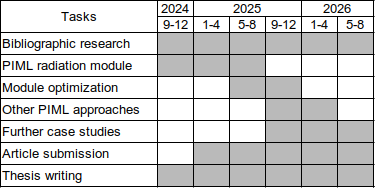
\includegraphics[width=.8\columnwidth]{schedule}
\label{fig:schedule}
\end{figure}



%========================================
\section*{Acknowledgment}
%========================================

Authors thank LNCC (National Laboratory for Scientific Computing) for grant 205341 AMPEMI (call 2020-I), which allows access to the Santos Dumont supercomputer (node of the SINAPAD, the Brazilian HPC system). This study was financed in part by the Coordination for the Improvement of Higher Education Personnel (CAPES), Brazil, finance Code 001, and also by the CNPq Project 446053/2023-6. The authors also thank the Brazilian Ministry of Science, Technology and Innovation, and the Brazilian Space Agency. %% 4o capítulo

%% insira quantos capítulos desejar com o seguinte comando:
%\include{_pasta_do_arquivo_/_meu_arquivo_} %%sem a extensão
%% note que deverá haver um arquivo _meu_arquivo_.tex (com extensão) no diretório _pasta_do_arquivo_

%% Bibliografia %% não alterar %% obrigatório %testebib
\bibliography{./refs} %% aponte para seu arquivo de bibliografia no formato bibtex (p.ex: referencia.bib)

%\include{./docs/09_glossario} %% insira os termos do glossário no arquivo glossario.tex %% opcional

%% opcional, comente esta linha e a seguintes se não houver apendice(s)
% \inicioApendice 
% \include{./docs/10_01_apendice1} %% insira apendices tal qual capítulos acima

% \inicioAnexo
% \include{./docs/11_01_anexo1}
% \include{./docs/11_02_anexo2}
% \include{./docs/11_03_anexo3}

\inicioIndice
%%%%%%%%%%%%%%%%%%%%%%%%%%%%%%%%%%%%%%%%%%%%%%%%%%%%%%
%Contracapa
%%%%%%%%%%%%%%%%%%%%%%%%%%%%%%%%%%%%%%%%%%%%%%%%%%%%%%

\thispagestyle{empty}
 \begin{table}
  \begin{center}
  \begin{tabularx}{\textwidth}{X}
   \textbf{PUBLICAÇÕES TÉCNICO-CIENTÍFICAS EDITADAS PELO INPE}
  \end{tabularx} 
  \end{center}
 \end{table}
  
 \begin{table}
  \begin{center}
  \begin{tabularx}{\textwidth}{X X}
      
  \textbf{Teses e Dissertações (TDI)}              & \textbf{Manuais Técnicos (MAN)}\\
\\
Teses e Dissertações apresentadas nos Cursos de Pós-Graduação do INPE.	&
São publicações de caráter técnico que incluem normas, procedimentos, instruções e orientações.\\
\\
\textbf{Notas Técnico-Científicas (NTC)}           & \textbf{Relatórios de Pesquisa (RPQ)}\\
\\
Incluem resultados preliminares de pesquisa, descrição de equipamentos, descrição e/ou documentação de programas de computador, descrição de sistemas e experimentos, apresentação de testes, dados, atlas, e documentação de projetos de engenharia. 
&	
Reportam resultados ou progressos de pesquisas tanto de natureza técnica quanto científica, cujo nível seja compatível com o de uma publicação em periódico nacional ou internacional.\\
\\
\textbf{Propostas e Relatórios de Projetos (PRP)}	& \textbf{Publicações Didáticas (PUD)} 
\\
\\
São propostas de projetos técnico-científicos e relatórios de acompanhamento de projetos, atividades e convênios.
&	
Incluem apostilas, notas de aula e manuais didáticos. \\
\\         
\textbf{Publicações Seriadas} 	& \textbf{Programas de Computador (PDC)}\\
\\
São os seriados técnico-científicos: boletins, periódicos, anuários e anais de eventos (simpósios e congressos). Constam destas publicações o Internacional Standard Serial Number (ISSN), que é um código único e definitivo para identificação de títulos de seriados. 
&	
São a sequência de instruções ou códigos, expressos em uma linguagem de programação compilada ou interpretada, a ser executada por um computador para alcançar um determinado objetivo. Aceitam-se tanto programas fonte quanto os executáveis.\\
\\
\textbf{Pré-publicações (PRE)} \\
\\
Todos os artigos publicados em  periódicos, anais e como capítulos de livros. \\                 \end{tabularx}
  \end{center}
 \end{table}


\end{document}